%%%%%%%%%%%%%%%%%%%%%%%%%%%%%%%%%%%%%%%%%%%%%%%%%%%%%%%%%%%%%%%%%%%%%%
% LaTeX Template: Beamer arrows
%
% Source: http://www.texample.net/
% Feel free to distribute this template, but please keep the
% referal to TeXample.net.
% Date: Nov 2006
% 
%%%%%%%%%%%%%%%%%%%%%%%%%%%%%%%%%%%%%%%%%%%%%%%%%%%%%%%%%%%%%%%%%%%%%%

\documentclass{beamer} %
\usepackage[spanish]{babel}
\usetheme{CambridgeUS}
\usepackage[utf8x]{inputenc}
\usefonttheme{professionalfonts}
\usepackage{times}
\usepackage{tikz}
\usepackage{amsmath}
\usepackage{verbatim}
\usetikzlibrary{arrows,shapes}
\usepackage{natbib}
\usepackage{booktabs}

\bibliographystyle{../report/apalike_es}
\graphicspath{../report/imagenes}
\newcommand{\mono}[1]{{\ttfamily #1}}

\author{Luis Guillermo Cornejo Suárez}
\institute[UCR]{Universidad de Costa Rica}
\title[PRIS-Lab Motion analysis Software]{Desarrollo de un \emph{software framework} para el análisis de variables cinemáticas y espacio-temporales de la marcha.}
\date{viernes 12 de agosto del 2016}


\begin{document}

\begin{frame}
    \titlepage
\end{frame}

%================================================================
\section{Introducción}

\begin{frame}{¿Qué es la marcha?}
   \begin{block}{Definición}
   Por marcha se entiende el acto de desplazarse utilizando las extremidades corporales inferiores. 
   \end{block}
\end{frame}

\begin{frame}{¿Qué es la marcha?}
    Según \citep{menz} la marcha consiste de cuatro tareas:
    \begin{itemize}
        \item Inicio y terminación de los movimientos locomotores.
        \item Generación de movimientos continuos para desplazarse hacia adelante.
        \item Mantenimiento del equilibrio .
        \item Adaptabilidad al ambiente. 
    \end{itemize}
    Se puede estudiar desde la \emph{dinámica} y la \emph{cinemática}
\end{frame}

\begin{frame}{Ciclo de la marcha}
    \begin{figure}
        \centering
        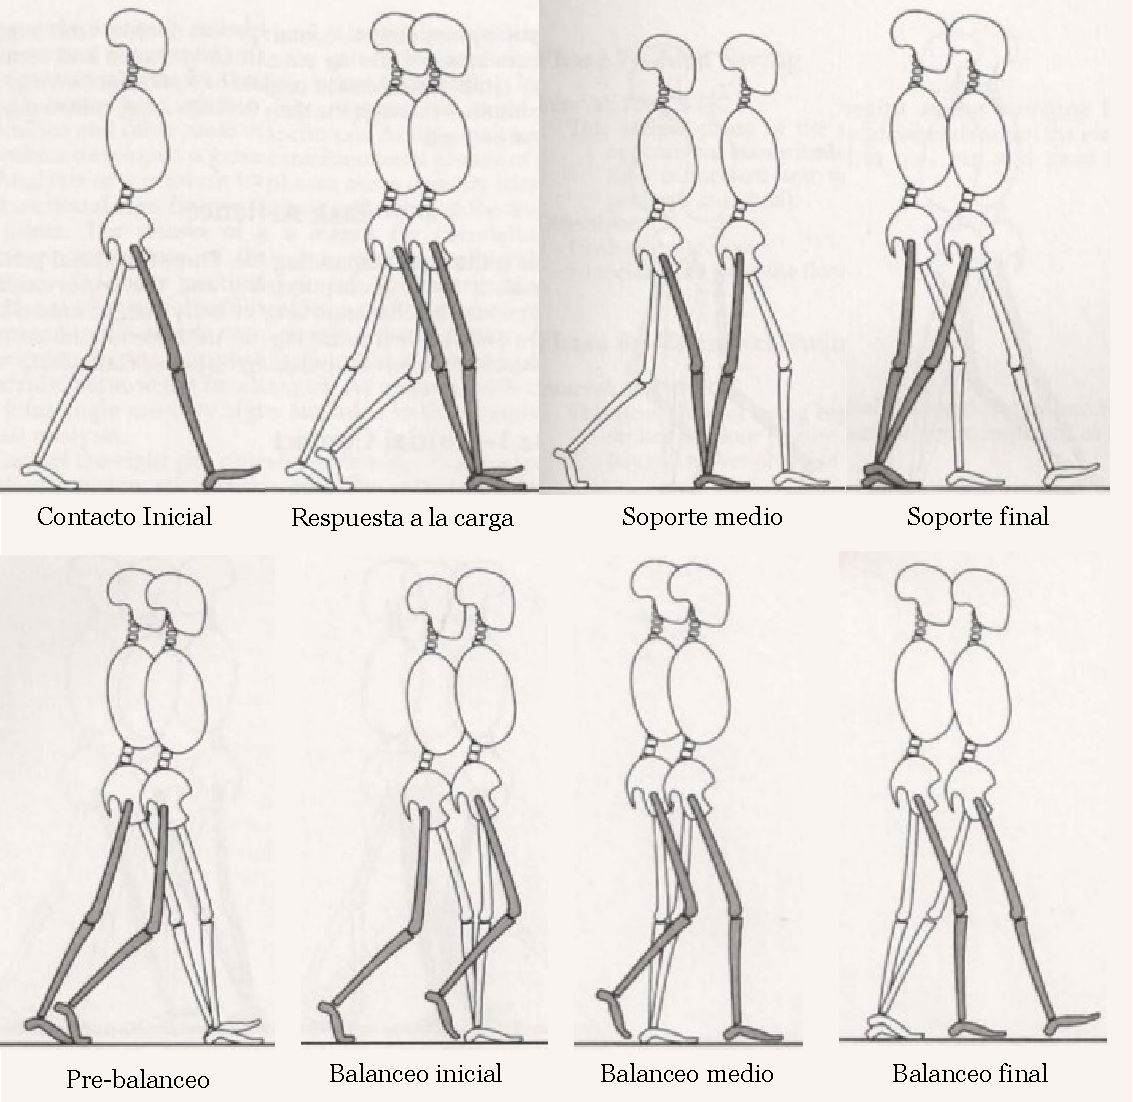
\includegraphics[height=0.7\textheight]{../report/imagenes/ciclo_marcha}
        \caption{Ilustración del ciclo de la marcha, tomado de \citep{perry}}
    \end{figure}
\end{frame}

\begin{frame}{Patrón de la marcha}
        % GNUPLOT: LaTeX picture
\setlength{\unitlength}{0.240900pt}
\ifx\plotpoint\undefined\newsavebox{\plotpoint}\fi
\begin{picture}(1500,900)(0,0)
\sbox{\plotpoint}{\rule[-0.200pt]{0.400pt}{0.400pt}}%
\put(191.0,131.0){\rule[-0.200pt]{4.818pt}{0.400pt}}
\put(171,131){\makebox(0,0)[r]{ 0.05}}
\put(1419.0,131.0){\rule[-0.200pt]{4.818pt}{0.400pt}}
\put(191.0,239.0){\rule[-0.200pt]{4.818pt}{0.400pt}}
\put(171,239){\makebox(0,0)[r]{ 0.1}}
\put(1419.0,239.0){\rule[-0.200pt]{4.818pt}{0.400pt}}
\put(191.0,346.0){\rule[-0.200pt]{4.818pt}{0.400pt}}
\put(171,346){\makebox(0,0)[r]{ 0.15}}
\put(1419.0,346.0){\rule[-0.200pt]{4.818pt}{0.400pt}}
\put(191.0,454.0){\rule[-0.200pt]{4.818pt}{0.400pt}}
\put(171,454){\makebox(0,0)[r]{ 0.2}}
\put(1419.0,454.0){\rule[-0.200pt]{4.818pt}{0.400pt}}
\put(191.0,561.0){\rule[-0.200pt]{4.818pt}{0.400pt}}
\put(171,561){\makebox(0,0)[r]{ 0.25}}
\put(1419.0,561.0){\rule[-0.200pt]{4.818pt}{0.400pt}}
\put(191.0,669.0){\rule[-0.200pt]{4.818pt}{0.400pt}}
\put(171,669){\makebox(0,0)[r]{ 0.3}}
\put(1419.0,669.0){\rule[-0.200pt]{4.818pt}{0.400pt}}
\put(191.0,776.0){\rule[-0.200pt]{4.818pt}{0.400pt}}
\put(171,776){\makebox(0,0)[r]{ 0.35}}
\put(1419.0,776.0){\rule[-0.200pt]{4.818pt}{0.400pt}}
\put(333.0,131.0){\rule[-0.200pt]{0.400pt}{4.818pt}}
\put(333,90){\makebox(0,0){ 400}}
\put(333.0,756.0){\rule[-0.200pt]{0.400pt}{4.818pt}}
\put(542.0,131.0){\rule[-0.200pt]{0.400pt}{4.818pt}}
\put(542,90){\makebox(0,0){ 600}}
\put(542.0,756.0){\rule[-0.200pt]{0.400pt}{4.818pt}}
\put(752.0,131.0){\rule[-0.200pt]{0.400pt}{4.818pt}}
\put(752,90){\makebox(0,0){ 800}}
\put(752.0,756.0){\rule[-0.200pt]{0.400pt}{4.818pt}}
\put(962.0,131.0){\rule[-0.200pt]{0.400pt}{4.818pt}}
\put(962,90){\makebox(0,0){ 1000}}
\put(962.0,756.0){\rule[-0.200pt]{0.400pt}{4.818pt}}
\put(1172.0,131.0){\rule[-0.200pt]{0.400pt}{4.818pt}}
\put(1172,90){\makebox(0,0){ 1200}}
\put(1172.0,756.0){\rule[-0.200pt]{0.400pt}{4.818pt}}
\put(1381.0,131.0){\rule[-0.200pt]{0.400pt}{4.818pt}}
\put(1381,90){\makebox(0,0){ 1400}}
\put(1381.0,756.0){\rule[-0.200pt]{0.400pt}{4.818pt}}
\put(191.0,131.0){\rule[-0.200pt]{0.400pt}{155.380pt}}
\put(191.0,131.0){\rule[-0.200pt]{300.643pt}{0.400pt}}
\put(1439.0,131.0){\rule[-0.200pt]{0.400pt}{155.380pt}}
\put(191.0,776.0){\rule[-0.200pt]{300.643pt}{0.400pt}}
\put(30,453){\makebox(0,0){\rotatebox{90}{Altura (m)}}}
\put(815,29){\makebox(0,0){Frames}}
\put(815,838){\makebox(0,0){Altura del talon}}
\put(191,237){\rule{1pt}{1pt}}
\put(192,237){\rule{1pt}{1pt}}
\put(193,236){\rule{1pt}{1pt}}
\put(194,236){\rule{1pt}{1pt}}
\put(195,235){\rule{1pt}{1pt}}
\put(196,234){\rule{1pt}{1pt}}
\put(197,234){\rule{1pt}{1pt}}
\put(198,233){\rule{1pt}{1pt}}
\put(199,233){\rule{1pt}{1pt}}
\put(200,233){\rule{1pt}{1pt}}
\put(201,233){\rule{1pt}{1pt}}
\put(203,233){\rule{1pt}{1pt}}
\put(204,233){\rule{1pt}{1pt}}
\put(205,234){\rule{1pt}{1pt}}
\put(206,234){\rule{1pt}{1pt}}
\put(207,234){\rule{1pt}{1pt}}
\put(208,235){\rule{1pt}{1pt}}
\put(209,235){\rule{1pt}{1pt}}
\put(210,235){\rule{1pt}{1pt}}
\put(211,236){\rule{1pt}{1pt}}
\put(212,236){\rule{1pt}{1pt}}
\put(213,237){\rule{1pt}{1pt}}
\put(214,237){\rule{1pt}{1pt}}
\put(215,238){\rule{1pt}{1pt}}
\put(216,238){\rule{1pt}{1pt}}
\put(217,239){\rule{1pt}{1pt}}
\put(218,239){\rule{1pt}{1pt}}
\put(219,240){\rule{1pt}{1pt}}
\put(220,240){\rule{1pt}{1pt}}
\put(221,241){\rule{1pt}{1pt}}
\put(222,241){\rule{1pt}{1pt}}
\put(224,242){\rule{1pt}{1pt}}
\put(225,241){\rule{1pt}{1pt}}
\put(226,242){\rule{1pt}{1pt}}
\put(227,242){\rule{1pt}{1pt}}
\put(228,242){\rule{1pt}{1pt}}
\put(229,242){\rule{1pt}{1pt}}
\put(230,242){\rule{1pt}{1pt}}
\put(231,243){\rule{1pt}{1pt}}
\put(232,243){\rule{1pt}{1pt}}
\put(233,243){\rule{1pt}{1pt}}
\put(234,242){\rule{1pt}{1pt}}
\put(235,243){\rule{1pt}{1pt}}
\put(236,243){\rule{1pt}{1pt}}
\put(237,244){\rule{1pt}{1pt}}
\put(238,244){\rule{1pt}{1pt}}
\put(239,244){\rule{1pt}{1pt}}
\put(240,244){\rule{1pt}{1pt}}
\put(241,244){\rule{1pt}{1pt}}
\put(242,245){\rule{1pt}{1pt}}
\put(243,245){\rule{1pt}{1pt}}
\put(244,246){\rule{1pt}{1pt}}
\put(246,247){\rule{1pt}{1pt}}
\put(247,245){\rule{1pt}{1pt}}
\put(248,247){\rule{1pt}{1pt}}
\put(249,249){\rule{1pt}{1pt}}
\put(250,248){\rule{1pt}{1pt}}
\put(251,251){\rule{1pt}{1pt}}
\put(252,248){\rule{1pt}{1pt}}
\put(253,249){\rule{1pt}{1pt}}
\put(254,249){\rule{1pt}{1pt}}
\put(255,244){\rule{1pt}{1pt}}
\put(256,250){\rule{1pt}{1pt}}
\put(257,250){\rule{1pt}{1pt}}
\put(258,248){\rule{1pt}{1pt}}
\put(259,249){\rule{1pt}{1pt}}
\put(260,249){\rule{1pt}{1pt}}
\put(261,256){\rule{1pt}{1pt}}
\put(262,253){\rule{1pt}{1pt}}
\put(263,249){\rule{1pt}{1pt}}
\put(264,252){\rule{1pt}{1pt}}
\put(265,252){\rule{1pt}{1pt}}
\put(267,253){\rule{1pt}{1pt}}
\put(268,253){\rule{1pt}{1pt}}
\put(269,254){\rule{1pt}{1pt}}
\put(270,255){\rule{1pt}{1pt}}
\put(271,257){\rule{1pt}{1pt}}
\put(272,258){\rule{1pt}{1pt}}
\put(273,259){\rule{1pt}{1pt}}
\put(274,260){\rule{1pt}{1pt}}
\put(275,262){\rule{1pt}{1pt}}
\put(276,264){\rule{1pt}{1pt}}
\put(277,266){\rule{1pt}{1pt}}
\put(278,268){\rule{1pt}{1pt}}
\put(279,270){\rule{1pt}{1pt}}
\put(280,273){\rule{1pt}{1pt}}
\put(281,276){\rule{1pt}{1pt}}
\put(282,278){\rule{1pt}{1pt}}
\put(283,281){\rule{1pt}{1pt}}
\put(284,285){\rule{1pt}{1pt}}
\put(285,288){\rule{1pt}{1pt}}
\put(286,292){\rule{1pt}{1pt}}
\put(287,296){\rule{1pt}{1pt}}
\put(289,300){\rule{1pt}{1pt}}
\put(290,304){\rule{1pt}{1pt}}
\put(291,308){\rule{1pt}{1pt}}
\put(292,313){\rule{1pt}{1pt}}
\put(293,318){\rule{1pt}{1pt}}
\put(294,324){\rule{1pt}{1pt}}
\put(295,329){\rule{1pt}{1pt}}
\put(296,335){\rule{1pt}{1pt}}
\put(297,341){\rule{1pt}{1pt}}
\put(298,347){\rule{1pt}{1pt}}
\put(299,353){\rule{1pt}{1pt}}
\put(300,359){\rule{1pt}{1pt}}
\put(301,365){\rule{1pt}{1pt}}
\put(302,372){\rule{1pt}{1pt}}
\put(303,379){\rule{1pt}{1pt}}
\put(304,385){\rule{1pt}{1pt}}
\put(305,392){\rule{1pt}{1pt}}
\put(306,399){\rule{1pt}{1pt}}
\put(307,406){\rule{1pt}{1pt}}
\put(308,413){\rule{1pt}{1pt}}
\put(310,420){\rule{1pt}{1pt}}
\put(311,427){\rule{1pt}{1pt}}
\put(312,434){\rule{1pt}{1pt}}
\put(313,442){\rule{1pt}{1pt}}
\put(314,449){\rule{1pt}{1pt}}
\put(315,457){\rule{1pt}{1pt}}
\put(316,465){\rule{1pt}{1pt}}
\put(317,473){\rule{1pt}{1pt}}
\put(318,481){\rule{1pt}{1pt}}
\put(319,490){\rule{1pt}{1pt}}
\put(320,499){\rule{1pt}{1pt}}
\put(321,508){\rule{1pt}{1pt}}
\put(322,517){\rule{1pt}{1pt}}
\put(323,525){\rule{1pt}{1pt}}
\put(324,533){\rule{1pt}{1pt}}
\put(325,541){\rule{1pt}{1pt}}
\put(326,551){\rule{1pt}{1pt}}
\put(327,560){\rule{1pt}{1pt}}
\put(328,568){\rule{1pt}{1pt}}
\put(329,575){\rule{1pt}{1pt}}
\put(330,583){\rule{1pt}{1pt}}
\put(332,590){\rule{1pt}{1pt}}
\put(333,596){\rule{1pt}{1pt}}
\put(334,602){\rule{1pt}{1pt}}
\put(335,608){\rule{1pt}{1pt}}
\put(336,612){\rule{1pt}{1pt}}
\put(337,615){\rule{1pt}{1pt}}
\put(338,618){\rule{1pt}{1pt}}
\put(339,619){\rule{1pt}{1pt}}
\put(340,620){\rule{1pt}{1pt}}
\put(341,620){\rule{1pt}{1pt}}
\put(342,619){\rule{1pt}{1pt}}
\put(343,618){\rule{1pt}{1pt}}
\put(344,616){\rule{1pt}{1pt}}
\put(345,613){\rule{1pt}{1pt}}
\put(346,610){\rule{1pt}{1pt}}
\put(347,606){\rule{1pt}{1pt}}
\put(348,601){\rule{1pt}{1pt}}
\put(349,596){\rule{1pt}{1pt}}
\put(350,589){\rule{1pt}{1pt}}
\put(351,583){\rule{1pt}{1pt}}
\put(353,576){\rule{1pt}{1pt}}
\put(354,569){\rule{1pt}{1pt}}
\put(355,561){\rule{1pt}{1pt}}
\put(356,553){\rule{1pt}{1pt}}
\put(357,545){\rule{1pt}{1pt}}
\put(358,536){\rule{1pt}{1pt}}
\put(359,528){\rule{1pt}{1pt}}
\put(360,519){\rule{1pt}{1pt}}
\put(361,511){\rule{1pt}{1pt}}
\put(362,502){\rule{1pt}{1pt}}
\put(363,493){\rule{1pt}{1pt}}
\put(364,484){\rule{1pt}{1pt}}
\put(365,474){\rule{1pt}{1pt}}
\put(366,464){\rule{1pt}{1pt}}
\put(367,455){\rule{1pt}{1pt}}
\put(368,446){\rule{1pt}{1pt}}
\put(369,436){\rule{1pt}{1pt}}
\put(370,427){\rule{1pt}{1pt}}
\put(371,418){\rule{1pt}{1pt}}
\put(372,409){\rule{1pt}{1pt}}
\put(373,401){\rule{1pt}{1pt}}
\put(375,392){\rule{1pt}{1pt}}
\put(376,384){\rule{1pt}{1pt}}
\put(377,376){\rule{1pt}{1pt}}
\put(378,368){\rule{1pt}{1pt}}
\put(379,360){\rule{1pt}{1pt}}
\put(380,352){\rule{1pt}{1pt}}
\put(381,345){\rule{1pt}{1pt}}
\put(382,339){\rule{1pt}{1pt}}
\put(383,332){\rule{1pt}{1pt}}
\put(384,325){\rule{1pt}{1pt}}
\put(385,319){\rule{1pt}{1pt}}
\put(386,313){\rule{1pt}{1pt}}
\put(387,308){\rule{1pt}{1pt}}
\put(388,303){\rule{1pt}{1pt}}
\put(389,299){\rule{1pt}{1pt}}
\put(390,294){\rule{1pt}{1pt}}
\put(391,290){\rule{1pt}{1pt}}
\put(392,287){\rule{1pt}{1pt}}
\put(393,284){\rule{1pt}{1pt}}
\put(394,281){\rule{1pt}{1pt}}
\put(396,279){\rule{1pt}{1pt}}
\put(397,277){\rule{1pt}{1pt}}
\put(398,275){\rule{1pt}{1pt}}
\put(399,273){\rule{1pt}{1pt}}
\put(400,273){\rule{1pt}{1pt}}
\put(401,272){\rule{1pt}{1pt}}
\put(402,272){\rule{1pt}{1pt}}
\put(403,272){\rule{1pt}{1pt}}
\put(404,272){\rule{1pt}{1pt}}
\put(405,273){\rule{1pt}{1pt}}
\put(406,274){\rule{1pt}{1pt}}
\put(407,275){\rule{1pt}{1pt}}
\put(408,277){\rule{1pt}{1pt}}
\put(409,278){\rule{1pt}{1pt}}
\put(410,280){\rule{1pt}{1pt}}
\put(411,282){\rule{1pt}{1pt}}
\put(412,284){\rule{1pt}{1pt}}
\put(413,286){\rule{1pt}{1pt}}
\put(414,288){\rule{1pt}{1pt}}
\put(415,289){\rule{1pt}{1pt}}
\put(416,291){\rule{1pt}{1pt}}
\put(418,292){\rule{1pt}{1pt}}
\put(419,293){\rule{1pt}{1pt}}
\put(420,294){\rule{1pt}{1pt}}
\put(421,294){\rule{1pt}{1pt}}
\put(422,293){\rule{1pt}{1pt}}
\put(423,293){\rule{1pt}{1pt}}
\put(424,291){\rule{1pt}{1pt}}
\put(425,290){\rule{1pt}{1pt}}
\put(426,288){\rule{1pt}{1pt}}
\put(427,285){\rule{1pt}{1pt}}
\put(428,282){\rule{1pt}{1pt}}
\put(429,279){\rule{1pt}{1pt}}
\put(430,276){\rule{1pt}{1pt}}
\put(431,272){\rule{1pt}{1pt}}
\put(432,268){\rule{1pt}{1pt}}
\put(433,264){\rule{1pt}{1pt}}
\put(434,260){\rule{1pt}{1pt}}
\put(435,255){\rule{1pt}{1pt}}
\put(436,251){\rule{1pt}{1pt}}
\put(437,248){\rule{1pt}{1pt}}
\put(439,245){\rule{1pt}{1pt}}
\put(440,242){\rule{1pt}{1pt}}
\put(441,240){\rule{1pt}{1pt}}
\put(442,237){\rule{1pt}{1pt}}
\put(443,235){\rule{1pt}{1pt}}
\put(444,232){\rule{1pt}{1pt}}
\put(445,231){\rule{1pt}{1pt}}
\put(446,229){\rule{1pt}{1pt}}
\put(447,227){\rule{1pt}{1pt}}
\put(448,226){\rule{1pt}{1pt}}
\put(449,225){\rule{1pt}{1pt}}
\put(450,224){\rule{1pt}{1pt}}
\put(451,223){\rule{1pt}{1pt}}
\put(452,222){\rule{1pt}{1pt}}
\put(453,222){\rule{1pt}{1pt}}
\put(454,222){\rule{1pt}{1pt}}
\put(455,222){\rule{1pt}{1pt}}
\put(456,222){\rule{1pt}{1pt}}
\put(457,222){\rule{1pt}{1pt}}
\put(458,222){\rule{1pt}{1pt}}
\put(459,222){\rule{1pt}{1pt}}
\put(461,222){\rule{1pt}{1pt}}
\put(462,222){\rule{1pt}{1pt}}
\put(463,222){\rule{1pt}{1pt}}
\put(464,222){\rule{1pt}{1pt}}
\put(465,222){\rule{1pt}{1pt}}
\put(466,222){\rule{1pt}{1pt}}
\put(467,222){\rule{1pt}{1pt}}
\put(468,222){\rule{1pt}{1pt}}
\put(469,222){\rule{1pt}{1pt}}
\put(470,221){\rule{1pt}{1pt}}
\put(471,221){\rule{1pt}{1pt}}
\put(472,221){\rule{1pt}{1pt}}
\put(473,222){\rule{1pt}{1pt}}
\put(474,221){\rule{1pt}{1pt}}
\put(475,222){\rule{1pt}{1pt}}
\put(476,222){\rule{1pt}{1pt}}
\put(477,222){\rule{1pt}{1pt}}
\put(478,223){\rule{1pt}{1pt}}
\put(479,223){\rule{1pt}{1pt}}
\put(480,224){\rule{1pt}{1pt}}
\put(482,224){\rule{1pt}{1pt}}
\put(483,225){\rule{1pt}{1pt}}
\put(484,226){\rule{1pt}{1pt}}
\put(485,227){\rule{1pt}{1pt}}
\put(486,227){\rule{1pt}{1pt}}
\put(487,228){\rule{1pt}{1pt}}
\put(488,229){\rule{1pt}{1pt}}
\put(489,230){\rule{1pt}{1pt}}
\put(490,231){\rule{1pt}{1pt}}
\put(491,232){\rule{1pt}{1pt}}
\put(492,233){\rule{1pt}{1pt}}
\put(493,234){\rule{1pt}{1pt}}
\put(494,234){\rule{1pt}{1pt}}
\put(495,235){\rule{1pt}{1pt}}
\put(496,236){\rule{1pt}{1pt}}
\put(497,237){\rule{1pt}{1pt}}
\put(498,238){\rule{1pt}{1pt}}
\put(499,239){\rule{1pt}{1pt}}
\put(500,239){\rule{1pt}{1pt}}
\put(501,240){\rule{1pt}{1pt}}
\put(502,241){\rule{1pt}{1pt}}
\put(504,241){\rule{1pt}{1pt}}
\put(505,242){\rule{1pt}{1pt}}
\put(506,243){\rule{1pt}{1pt}}
\put(507,243){\rule{1pt}{1pt}}
\put(508,244){\rule{1pt}{1pt}}
\put(509,245){\rule{1pt}{1pt}}
\put(510,245){\rule{1pt}{1pt}}
\put(511,246){\rule{1pt}{1pt}}
\put(512,247){\rule{1pt}{1pt}}
\put(513,247){\rule{1pt}{1pt}}
\put(514,248){\rule{1pt}{1pt}}
\put(515,248){\rule{1pt}{1pt}}
\put(516,249){\rule{1pt}{1pt}}
\put(517,249){\rule{1pt}{1pt}}
\put(518,250){\rule{1pt}{1pt}}
\put(519,250){\rule{1pt}{1pt}}
\put(520,251){\rule{1pt}{1pt}}
\put(521,251){\rule{1pt}{1pt}}
\put(522,252){\rule{1pt}{1pt}}
\put(523,252){\rule{1pt}{1pt}}
\put(524,253){\rule{1pt}{1pt}}
\put(526,253){\rule{1pt}{1pt}}
\put(527,253){\rule{1pt}{1pt}}
\put(528,254){\rule{1pt}{1pt}}
\put(529,255){\rule{1pt}{1pt}}
\put(530,255){\rule{1pt}{1pt}}
\put(531,256){\rule{1pt}{1pt}}
\put(532,257){\rule{1pt}{1pt}}
\put(533,257){\rule{1pt}{1pt}}
\put(534,258){\rule{1pt}{1pt}}
\put(535,259){\rule{1pt}{1pt}}
\put(536,261){\rule{1pt}{1pt}}
\put(537,262){\rule{1pt}{1pt}}
\put(538,264){\rule{1pt}{1pt}}
\put(539,265){\rule{1pt}{1pt}}
\put(540,268){\rule{1pt}{1pt}}
\put(541,270){\rule{1pt}{1pt}}
\put(542,273){\rule{1pt}{1pt}}
\put(543,276){\rule{1pt}{1pt}}
\put(544,279){\rule{1pt}{1pt}}
\put(545,282){\rule{1pt}{1pt}}
\put(547,286){\rule{1pt}{1pt}}
\put(548,290){\rule{1pt}{1pt}}
\put(549,295){\rule{1pt}{1pt}}
\put(550,299){\rule{1pt}{1pt}}
\put(551,305){\rule{1pt}{1pt}}
\put(552,310){\rule{1pt}{1pt}}
\put(553,316){\rule{1pt}{1pt}}
\put(554,322){\rule{1pt}{1pt}}
\put(555,328){\rule{1pt}{1pt}}
\put(556,334){\rule{1pt}{1pt}}
\put(557,341){\rule{1pt}{1pt}}
\put(558,348){\rule{1pt}{1pt}}
\put(559,355){\rule{1pt}{1pt}}
\put(560,362){\rule{1pt}{1pt}}
\put(561,369){\rule{1pt}{1pt}}
\put(562,377){\rule{1pt}{1pt}}
\put(563,384){\rule{1pt}{1pt}}
\put(564,392){\rule{1pt}{1pt}}
\put(565,400){\rule{1pt}{1pt}}
\put(566,408){\rule{1pt}{1pt}}
\put(567,416){\rule{1pt}{1pt}}
\put(569,424){\rule{1pt}{1pt}}
\put(570,432){\rule{1pt}{1pt}}
\put(571,440){\rule{1pt}{1pt}}
\put(572,448){\rule{1pt}{1pt}}
\put(573,456){\rule{1pt}{1pt}}
\put(574,464){\rule{1pt}{1pt}}
\put(575,473){\rule{1pt}{1pt}}
\put(576,481){\rule{1pt}{1pt}}
\put(577,490){\rule{1pt}{1pt}}
\put(578,500){\rule{1pt}{1pt}}
\put(579,510){\rule{1pt}{1pt}}
\put(580,520){\rule{1pt}{1pt}}
\put(581,530){\rule{1pt}{1pt}}
\put(582,540){\rule{1pt}{1pt}}
\put(583,548){\rule{1pt}{1pt}}
\put(584,558){\rule{1pt}{1pt}}
\put(585,568){\rule{1pt}{1pt}}
\put(586,577){\rule{1pt}{1pt}}
\put(587,586){\rule{1pt}{1pt}}
\put(588,595){\rule{1pt}{1pt}}
\put(590,604){\rule{1pt}{1pt}}
\put(591,613){\rule{1pt}{1pt}}
\put(592,622){\rule{1pt}{1pt}}
\put(593,630){\rule{1pt}{1pt}}
\put(594,638){\rule{1pt}{1pt}}
\put(595,645){\rule{1pt}{1pt}}
\put(596,651){\rule{1pt}{1pt}}
\put(597,656){\rule{1pt}{1pt}}
\put(598,660){\rule{1pt}{1pt}}
\put(599,664){\rule{1pt}{1pt}}
\put(600,667){\rule{1pt}{1pt}}
\put(601,669){\rule{1pt}{1pt}}
\put(602,670){\rule{1pt}{1pt}}
\put(603,671){\rule{1pt}{1pt}}
\put(604,671){\rule{1pt}{1pt}}
\put(605,670){\rule{1pt}{1pt}}
\put(606,669){\rule{1pt}{1pt}}
\put(607,667){\rule{1pt}{1pt}}
\put(608,665){\rule{1pt}{1pt}}
\put(609,661){\rule{1pt}{1pt}}
\put(610,657){\rule{1pt}{1pt}}
\put(612,653){\rule{1pt}{1pt}}
\put(613,648){\rule{1pt}{1pt}}
\put(614,643){\rule{1pt}{1pt}}
\put(615,637){\rule{1pt}{1pt}}
\put(616,630){\rule{1pt}{1pt}}
\put(617,623){\rule{1pt}{1pt}}
\put(618,616){\rule{1pt}{1pt}}
\put(619,608){\rule{1pt}{1pt}}
\put(620,599){\rule{1pt}{1pt}}
\put(621,591){\rule{1pt}{1pt}}
\put(622,581){\rule{1pt}{1pt}}
\put(623,572){\rule{1pt}{1pt}}
\put(624,563){\rule{1pt}{1pt}}
\put(625,554){\rule{1pt}{1pt}}
\put(626,544){\rule{1pt}{1pt}}
\put(627,534){\rule{1pt}{1pt}}
\put(628,525){\rule{1pt}{1pt}}
\put(629,515){\rule{1pt}{1pt}}
\put(630,505){\rule{1pt}{1pt}}
\put(631,495){\rule{1pt}{1pt}}
\put(633,485){\rule{1pt}{1pt}}
\put(634,474){\rule{1pt}{1pt}}
\put(635,464){\rule{1pt}{1pt}}
\put(636,454){\rule{1pt}{1pt}}
\put(637,443){\rule{1pt}{1pt}}
\put(638,433){\rule{1pt}{1pt}}
\put(639,423){\rule{1pt}{1pt}}
\put(640,413){\rule{1pt}{1pt}}
\put(641,403){\rule{1pt}{1pt}}
\put(642,394){\rule{1pt}{1pt}}
\put(643,384){\rule{1pt}{1pt}}
\put(644,375){\rule{1pt}{1pt}}
\put(645,366){\rule{1pt}{1pt}}
\put(646,357){\rule{1pt}{1pt}}
\put(647,348){\rule{1pt}{1pt}}
\put(648,340){\rule{1pt}{1pt}}
\put(649,331){\rule{1pt}{1pt}}
\put(650,324){\rule{1pt}{1pt}}
\put(651,317){\rule{1pt}{1pt}}
\put(652,310){\rule{1pt}{1pt}}
\put(653,304){\rule{1pt}{1pt}}
\put(655,297){\rule{1pt}{1pt}}
\put(656,292){\rule{1pt}{1pt}}
\put(657,287){\rule{1pt}{1pt}}
\put(658,282){\rule{1pt}{1pt}}
\put(659,279){\rule{1pt}{1pt}}
\put(660,276){\rule{1pt}{1pt}}
\put(661,273){\rule{1pt}{1pt}}
\put(662,271){\rule{1pt}{1pt}}
\put(663,269){\rule{1pt}{1pt}}
\put(664,268){\rule{1pt}{1pt}}
\put(665,268){\rule{1pt}{1pt}}
\put(666,268){\rule{1pt}{1pt}}
\put(667,269){\rule{1pt}{1pt}}
\put(668,270){\rule{1pt}{1pt}}
\put(669,272){\rule{1pt}{1pt}}
\put(670,274){\rule{1pt}{1pt}}
\put(671,276){\rule{1pt}{1pt}}
\put(672,279){\rule{1pt}{1pt}}
\put(673,282){\rule{1pt}{1pt}}
\put(674,285){\rule{1pt}{1pt}}
\put(676,287){\rule{1pt}{1pt}}
\put(677,290){\rule{1pt}{1pt}}
\put(678,292){\rule{1pt}{1pt}}
\put(679,294){\rule{1pt}{1pt}}
\put(680,295){\rule{1pt}{1pt}}
\put(681,295){\rule{1pt}{1pt}}
\put(682,294){\rule{1pt}{1pt}}
\put(683,293){\rule{1pt}{1pt}}
\put(684,291){\rule{1pt}{1pt}}
\put(685,288){\rule{1pt}{1pt}}
\put(686,284){\rule{1pt}{1pt}}
\put(687,280){\rule{1pt}{1pt}}
\put(688,276){\rule{1pt}{1pt}}
\put(689,271){\rule{1pt}{1pt}}
\put(690,266){\rule{1pt}{1pt}}
\put(691,261){\rule{1pt}{1pt}}
\put(692,256){\rule{1pt}{1pt}}
\put(693,251){\rule{1pt}{1pt}}
\put(694,245){\rule{1pt}{1pt}}
\put(695,241){\rule{1pt}{1pt}}
\put(696,236){\rule{1pt}{1pt}}
\put(698,233){\rule{1pt}{1pt}}
\put(699,229){\rule{1pt}{1pt}}
\put(700,227){\rule{1pt}{1pt}}
\put(701,224){\rule{1pt}{1pt}}
\put(702,220){\rule{1pt}{1pt}}
\put(703,217){\rule{1pt}{1pt}}
\put(704,214){\rule{1pt}{1pt}}
\put(705,213){\rule{1pt}{1pt}}
\put(706,211){\rule{1pt}{1pt}}
\put(707,209){\rule{1pt}{1pt}}
\put(708,208){\rule{1pt}{1pt}}
\put(709,209){\rule{1pt}{1pt}}
\put(710,209){\rule{1pt}{1pt}}
\put(711,209){\rule{1pt}{1pt}}
\put(712,209){\rule{1pt}{1pt}}
\put(713,210){\rule{1pt}{1pt}}
\put(714,210){\rule{1pt}{1pt}}
\put(715,210){\rule{1pt}{1pt}}
\put(716,210){\rule{1pt}{1pt}}
\put(717,210){\rule{1pt}{1pt}}
\put(719,210){\rule{1pt}{1pt}}
\put(720,210){\rule{1pt}{1pt}}
\put(721,210){\rule{1pt}{1pt}}
\put(722,209){\rule{1pt}{1pt}}
\put(723,209){\rule{1pt}{1pt}}
\put(724,209){\rule{1pt}{1pt}}
\put(725,209){\rule{1pt}{1pt}}
\put(726,209){\rule{1pt}{1pt}}
\put(727,209){\rule{1pt}{1pt}}
\put(728,209){\rule{1pt}{1pt}}
\put(729,209){\rule{1pt}{1pt}}
\put(730,209){\rule{1pt}{1pt}}
\put(731,210){\rule{1pt}{1pt}}
\put(732,210){\rule{1pt}{1pt}}
\put(733,211){\rule{1pt}{1pt}}
\put(734,211){\rule{1pt}{1pt}}
\put(735,212){\rule{1pt}{1pt}}
\put(736,213){\rule{1pt}{1pt}}
\put(737,213){\rule{1pt}{1pt}}
\put(738,214){\rule{1pt}{1pt}}
\put(739,215){\rule{1pt}{1pt}}
\put(741,216){\rule{1pt}{1pt}}
\put(742,216){\rule{1pt}{1pt}}
\put(743,217){\rule{1pt}{1pt}}
\put(744,217){\rule{1pt}{1pt}}
\put(745,218){\rule{1pt}{1pt}}
\put(746,219){\rule{1pt}{1pt}}
\put(747,220){\rule{1pt}{1pt}}
\put(748,221){\rule{1pt}{1pt}}
\put(749,222){\rule{1pt}{1pt}}
\put(750,223){\rule{1pt}{1pt}}
\put(751,224){\rule{1pt}{1pt}}
\put(752,226){\rule{1pt}{1pt}}
\put(753,227){\rule{1pt}{1pt}}
\put(754,228){\rule{1pt}{1pt}}
\put(755,229){\rule{1pt}{1pt}}
\put(756,230){\rule{1pt}{1pt}}
\put(757,231){\rule{1pt}{1pt}}
\put(758,232){\rule{1pt}{1pt}}
\put(759,233){\rule{1pt}{1pt}}
\put(760,234){\rule{1pt}{1pt}}
\put(762,236){\rule{1pt}{1pt}}
\put(763,237){\rule{1pt}{1pt}}
\put(764,238){\rule{1pt}{1pt}}
\put(765,239){\rule{1pt}{1pt}}
\put(766,240){\rule{1pt}{1pt}}
\put(767,241){\rule{1pt}{1pt}}
\put(768,242){\rule{1pt}{1pt}}
\put(769,243){\rule{1pt}{1pt}}
\put(770,244){\rule{1pt}{1pt}}
\put(771,244){\rule{1pt}{1pt}}
\put(772,245){\rule{1pt}{1pt}}
\put(773,246){\rule{1pt}{1pt}}
\put(774,247){\rule{1pt}{1pt}}
\put(775,247){\rule{1pt}{1pt}}
\put(776,248){\rule{1pt}{1pt}}
\put(777,248){\rule{1pt}{1pt}}
\put(778,249){\rule{1pt}{1pt}}
\put(779,249){\rule{1pt}{1pt}}
\put(780,250){\rule{1pt}{1pt}}
\put(781,250){\rule{1pt}{1pt}}
\put(782,251){\rule{1pt}{1pt}}
\put(784,252){\rule{1pt}{1pt}}
\put(785,252){\rule{1pt}{1pt}}
\put(786,253){\rule{1pt}{1pt}}
\put(787,253){\rule{1pt}{1pt}}
\put(788,254){\rule{1pt}{1pt}}
\put(789,255){\rule{1pt}{1pt}}
\put(790,256){\rule{1pt}{1pt}}
\put(791,257){\rule{1pt}{1pt}}
\put(792,259){\rule{1pt}{1pt}}
\put(793,260){\rule{1pt}{1pt}}
\put(794,262){\rule{1pt}{1pt}}
\put(795,264){\rule{1pt}{1pt}}
\put(796,266){\rule{1pt}{1pt}}
\put(797,268){\rule{1pt}{1pt}}
\put(798,270){\rule{1pt}{1pt}}
\put(799,273){\rule{1pt}{1pt}}
\put(800,276){\rule{1pt}{1pt}}
\put(801,279){\rule{1pt}{1pt}}
\put(802,283){\rule{1pt}{1pt}}
\put(803,286){\rule{1pt}{1pt}}
\put(805,291){\rule{1pt}{1pt}}
\put(806,296){\rule{1pt}{1pt}}
\put(807,300){\rule{1pt}{1pt}}
\put(808,306){\rule{1pt}{1pt}}
\put(809,311){\rule{1pt}{1pt}}
\put(810,317){\rule{1pt}{1pt}}
\put(811,323){\rule{1pt}{1pt}}
\put(812,329){\rule{1pt}{1pt}}
\put(813,335){\rule{1pt}{1pt}}
\put(814,342){\rule{1pt}{1pt}}
\put(815,349){\rule{1pt}{1pt}}
\put(816,356){\rule{1pt}{1pt}}
\put(817,364){\rule{1pt}{1pt}}
\put(818,372){\rule{1pt}{1pt}}
\put(819,379){\rule{1pt}{1pt}}
\put(820,387){\rule{1pt}{1pt}}
\put(821,395){\rule{1pt}{1pt}}
\put(822,403){\rule{1pt}{1pt}}
\put(823,410){\rule{1pt}{1pt}}
\put(824,418){\rule{1pt}{1pt}}
\put(825,426){\rule{1pt}{1pt}}
\put(827,434){\rule{1pt}{1pt}}
\put(828,442){\rule{1pt}{1pt}}
\put(829,450){\rule{1pt}{1pt}}
\put(830,458){\rule{1pt}{1pt}}
\put(831,466){\rule{1pt}{1pt}}
\put(832,475){\rule{1pt}{1pt}}
\put(833,484){\rule{1pt}{1pt}}
\put(834,492){\rule{1pt}{1pt}}
\put(835,501){\rule{1pt}{1pt}}
\put(836,510){\rule{1pt}{1pt}}
\put(837,519){\rule{1pt}{1pt}}
\put(838,527){\rule{1pt}{1pt}}
\put(839,535){\rule{1pt}{1pt}}
\put(840,546){\rule{1pt}{1pt}}
\put(841,554){\rule{1pt}{1pt}}
\put(842,563){\rule{1pt}{1pt}}
\put(843,571){\rule{1pt}{1pt}}
\put(844,579){\rule{1pt}{1pt}}
\put(845,586){\rule{1pt}{1pt}}
\put(846,594){\rule{1pt}{1pt}}
\put(848,602){\rule{1pt}{1pt}}
\put(849,609){\rule{1pt}{1pt}}
\put(850,615){\rule{1pt}{1pt}}
\put(851,621){\rule{1pt}{1pt}}
\put(852,626){\rule{1pt}{1pt}}
\put(853,630){\rule{1pt}{1pt}}
\put(854,633){\rule{1pt}{1pt}}
\put(855,636){\rule{1pt}{1pt}}
\put(856,638){\rule{1pt}{1pt}}
\put(857,639){\rule{1pt}{1pt}}
\put(858,640){\rule{1pt}{1pt}}
\put(859,640){\rule{1pt}{1pt}}
\put(860,640){\rule{1pt}{1pt}}
\put(861,639){\rule{1pt}{1pt}}
\put(862,637){\rule{1pt}{1pt}}
\put(863,635){\rule{1pt}{1pt}}
\put(864,631){\rule{1pt}{1pt}}
\put(865,628){\rule{1pt}{1pt}}
\put(866,623){\rule{1pt}{1pt}}
\put(867,619){\rule{1pt}{1pt}}
\put(868,613){\rule{1pt}{1pt}}
\put(870,608){\rule{1pt}{1pt}}
\put(871,602){\rule{1pt}{1pt}}
\put(872,595){\rule{1pt}{1pt}}
\put(873,588){\rule{1pt}{1pt}}
\put(874,580){\rule{1pt}{1pt}}
\put(875,573){\rule{1pt}{1pt}}
\put(876,564){\rule{1pt}{1pt}}
\put(877,556){\rule{1pt}{1pt}}
\put(878,546){\rule{1pt}{1pt}}
\put(879,537){\rule{1pt}{1pt}}
\put(880,529){\rule{1pt}{1pt}}
\put(881,519){\rule{1pt}{1pt}}
\put(882,510){\rule{1pt}{1pt}}
\put(883,501){\rule{1pt}{1pt}}
\put(884,492){\rule{1pt}{1pt}}
\put(885,482){\rule{1pt}{1pt}}
\put(886,473){\rule{1pt}{1pt}}
\put(887,464){\rule{1pt}{1pt}}
\put(888,454){\rule{1pt}{1pt}}
\put(889,445){\rule{1pt}{1pt}}
\put(891,435){\rule{1pt}{1pt}}
\put(892,426){\rule{1pt}{1pt}}
\put(893,417){\rule{1pt}{1pt}}
\put(894,407){\rule{1pt}{1pt}}
\put(895,398){\rule{1pt}{1pt}}
\put(896,389){\rule{1pt}{1pt}}
\put(897,380){\rule{1pt}{1pt}}
\put(898,372){\rule{1pt}{1pt}}
\put(899,363){\rule{1pt}{1pt}}
\put(900,355){\rule{1pt}{1pt}}
\put(901,347){\rule{1pt}{1pt}}
\put(902,340){\rule{1pt}{1pt}}
\put(903,332){\rule{1pt}{1pt}}
\put(904,325){\rule{1pt}{1pt}}
\put(905,319){\rule{1pt}{1pt}}
\put(906,312){\rule{1pt}{1pt}}
\put(907,306){\rule{1pt}{1pt}}
\put(908,301){\rule{1pt}{1pt}}
\put(909,295){\rule{1pt}{1pt}}
\put(910,291){\rule{1pt}{1pt}}
\put(911,287){\rule{1pt}{1pt}}
\put(913,283){\rule{1pt}{1pt}}
\put(914,280){\rule{1pt}{1pt}}
\put(915,277){\rule{1pt}{1pt}}
\put(916,275){\rule{1pt}{1pt}}
\put(917,273){\rule{1pt}{1pt}}
\put(918,272){\rule{1pt}{1pt}}
\put(919,271){\rule{1pt}{1pt}}
\put(920,271){\rule{1pt}{1pt}}
\put(921,272){\rule{1pt}{1pt}}
\put(922,272){\rule{1pt}{1pt}}
\put(923,274){\rule{1pt}{1pt}}
\put(924,275){\rule{1pt}{1pt}}
\put(925,277){\rule{1pt}{1pt}}
\put(926,280){\rule{1pt}{1pt}}
\put(927,283){\rule{1pt}{1pt}}
\put(928,285){\rule{1pt}{1pt}}
\put(929,289){\rule{1pt}{1pt}}
\put(930,292){\rule{1pt}{1pt}}
\put(931,295){\rule{1pt}{1pt}}
\put(932,298){\rule{1pt}{1pt}}
\put(934,301){\rule{1pt}{1pt}}
\put(935,304){\rule{1pt}{1pt}}
\put(936,307){\rule{1pt}{1pt}}
\put(937,309){\rule{1pt}{1pt}}
\put(938,310){\rule{1pt}{1pt}}
\put(939,311){\rule{1pt}{1pt}}
\put(940,311){\rule{1pt}{1pt}}
\put(941,311){\rule{1pt}{1pt}}
\put(942,310){\rule{1pt}{1pt}}
\put(943,308){\rule{1pt}{1pt}}
\put(944,306){\rule{1pt}{1pt}}
\put(945,303){\rule{1pt}{1pt}}
\put(946,299){\rule{1pt}{1pt}}
\put(947,295){\rule{1pt}{1pt}}
\put(948,291){\rule{1pt}{1pt}}
\put(949,286){\rule{1pt}{1pt}}
\put(950,281){\rule{1pt}{1pt}}
\put(951,276){\rule{1pt}{1pt}}
\put(952,270){\rule{1pt}{1pt}}
\put(953,265){\rule{1pt}{1pt}}
\put(954,259){\rule{1pt}{1pt}}
\put(956,253){\rule{1pt}{1pt}}
\put(957,248){\rule{1pt}{1pt}}
\put(958,243){\rule{1pt}{1pt}}
\put(959,238){\rule{1pt}{1pt}}
\put(960,234){\rule{1pt}{1pt}}
\put(961,230){\rule{1pt}{1pt}}
\put(962,226){\rule{1pt}{1pt}}
\put(963,222){\rule{1pt}{1pt}}
\put(964,218){\rule{1pt}{1pt}}
\put(965,214){\rule{1pt}{1pt}}
\put(966,210){\rule{1pt}{1pt}}
\put(967,208){\rule{1pt}{1pt}}
\put(968,206){\rule{1pt}{1pt}}
\put(969,205){\rule{1pt}{1pt}}
\put(970,204){\rule{1pt}{1pt}}
\put(971,203){\rule{1pt}{1pt}}
\put(972,203){\rule{1pt}{1pt}}
\put(973,203){\rule{1pt}{1pt}}
\put(974,204){\rule{1pt}{1pt}}
\put(975,204){\rule{1pt}{1pt}}
\put(977,205){\rule{1pt}{1pt}}
\put(978,205){\rule{1pt}{1pt}}
\put(979,205){\rule{1pt}{1pt}}
\put(980,205){\rule{1pt}{1pt}}
\put(981,206){\rule{1pt}{1pt}}
\put(982,206){\rule{1pt}{1pt}}
\put(983,206){\rule{1pt}{1pt}}
\put(984,206){\rule{1pt}{1pt}}
\put(985,206){\rule{1pt}{1pt}}
\put(986,206){\rule{1pt}{1pt}}
\put(987,206){\rule{1pt}{1pt}}
\put(988,206){\rule{1pt}{1pt}}
\put(989,205){\rule{1pt}{1pt}}
\put(990,205){\rule{1pt}{1pt}}
\put(991,206){\rule{1pt}{1pt}}
\put(992,206){\rule{1pt}{1pt}}
\put(993,206){\rule{1pt}{1pt}}
\put(994,206){\rule{1pt}{1pt}}
\put(995,207){\rule{1pt}{1pt}}
\put(996,207){\rule{1pt}{1pt}}
\put(997,208){\rule{1pt}{1pt}}
\put(999,209){\rule{1pt}{1pt}}
\put(1000,209){\rule{1pt}{1pt}}
\put(1001,210){\rule{1pt}{1pt}}
\put(1002,211){\rule{1pt}{1pt}}
\put(1003,212){\rule{1pt}{1pt}}
\put(1004,212){\rule{1pt}{1pt}}
\put(1005,213){\rule{1pt}{1pt}}
\put(1006,214){\rule{1pt}{1pt}}
\put(1007,215){\rule{1pt}{1pt}}
\put(1008,216){\rule{1pt}{1pt}}
\put(1009,217){\rule{1pt}{1pt}}
\put(1010,219){\rule{1pt}{1pt}}
\put(1011,220){\rule{1pt}{1pt}}
\put(1012,221){\rule{1pt}{1pt}}
\put(1013,223){\rule{1pt}{1pt}}
\put(1014,224){\rule{1pt}{1pt}}
\put(1015,225){\rule{1pt}{1pt}}
\put(1016,227){\rule{1pt}{1pt}}
\put(1017,228){\rule{1pt}{1pt}}
\put(1018,229){\rule{1pt}{1pt}}
\put(1020,230){\rule{1pt}{1pt}}
\put(1021,231){\rule{1pt}{1pt}}
\put(1022,233){\rule{1pt}{1pt}}
\put(1023,233){\rule{1pt}{1pt}}
\put(1024,234){\rule{1pt}{1pt}}
\put(1025,235){\rule{1pt}{1pt}}
\put(1026,236){\rule{1pt}{1pt}}
\put(1027,237){\rule{1pt}{1pt}}
\put(1028,237){\rule{1pt}{1pt}}
\put(1029,238){\rule{1pt}{1pt}}
\put(1030,238){\rule{1pt}{1pt}}
\put(1031,239){\rule{1pt}{1pt}}
\put(1032,239){\rule{1pt}{1pt}}
\put(1033,239){\rule{1pt}{1pt}}
\put(1034,240){\rule{1pt}{1pt}}
\put(1035,240){\rule{1pt}{1pt}}
\put(1036,240){\rule{1pt}{1pt}}
\put(1037,240){\rule{1pt}{1pt}}
\put(1038,240){\rule{1pt}{1pt}}
\put(1039,241){\rule{1pt}{1pt}}
\put(1040,241){\rule{1pt}{1pt}}
\put(1042,241){\rule{1pt}{1pt}}
\put(1043,241){\rule{1pt}{1pt}}
\put(1044,241){\rule{1pt}{1pt}}
\put(1045,242){\rule{1pt}{1pt}}
\put(1046,242){\rule{1pt}{1pt}}
\put(1047,242){\rule{1pt}{1pt}}
\put(1048,242){\rule{1pt}{1pt}}
\put(1049,243){\rule{1pt}{1pt}}
\put(1050,243){\rule{1pt}{1pt}}
\put(1051,244){\rule{1pt}{1pt}}
\put(1052,245){\rule{1pt}{1pt}}
\put(1053,245){\rule{1pt}{1pt}}
\put(1054,247){\rule{1pt}{1pt}}
\put(1055,247){\rule{1pt}{1pt}}
\put(1056,248){\rule{1pt}{1pt}}
\put(1057,250){\rule{1pt}{1pt}}
\put(1058,251){\rule{1pt}{1pt}}
\put(1059,253){\rule{1pt}{1pt}}
\put(1060,255){\rule{1pt}{1pt}}
\put(1061,257){\rule{1pt}{1pt}}
\put(1063,260){\rule{1pt}{1pt}}
\put(1064,262){\rule{1pt}{1pt}}
\put(1065,265){\rule{1pt}{1pt}}
\put(1066,269){\rule{1pt}{1pt}}
\put(1067,272){\rule{1pt}{1pt}}
\put(1068,276){\rule{1pt}{1pt}}
\put(1069,281){\rule{1pt}{1pt}}
\put(1070,286){\rule{1pt}{1pt}}
\put(1071,291){\rule{1pt}{1pt}}
\put(1072,296){\rule{1pt}{1pt}}
\put(1073,302){\rule{1pt}{1pt}}
\put(1074,308){\rule{1pt}{1pt}}
\put(1075,315){\rule{1pt}{1pt}}
\put(1076,322){\rule{1pt}{1pt}}
\put(1077,329){\rule{1pt}{1pt}}
\put(1078,337){\rule{1pt}{1pt}}
\put(1079,344){\rule{1pt}{1pt}}
\put(1080,352){\rule{1pt}{1pt}}
\put(1081,360){\rule{1pt}{1pt}}
\put(1082,369){\rule{1pt}{1pt}}
\put(1083,377){\rule{1pt}{1pt}}
\put(1085,386){\rule{1pt}{1pt}}
\put(1086,394){\rule{1pt}{1pt}}
\put(1087,403){\rule{1pt}{1pt}}
\put(1088,411){\rule{1pt}{1pt}}
\put(1089,420){\rule{1pt}{1pt}}
\put(1090,428){\rule{1pt}{1pt}}
\put(1091,436){\rule{1pt}{1pt}}
\put(1092,444){\rule{1pt}{1pt}}
\put(1093,453){\rule{1pt}{1pt}}
\put(1094,461){\rule{1pt}{1pt}}
\put(1095,471){\rule{1pt}{1pt}}
\put(1096,481){\rule{1pt}{1pt}}
\put(1097,490){\rule{1pt}{1pt}}
\put(1098,500){\rule{1pt}{1pt}}
\put(1099,510){\rule{1pt}{1pt}}
\put(1100,519){\rule{1pt}{1pt}}
\put(1101,529){\rule{1pt}{1pt}}
\put(1102,540){\rule{1pt}{1pt}}
\put(1103,550){\rule{1pt}{1pt}}
\put(1104,560){\rule{1pt}{1pt}}
\put(1106,570){\rule{1pt}{1pt}}
\put(1107,579){\rule{1pt}{1pt}}
\put(1108,588){\rule{1pt}{1pt}}
\put(1109,598){\rule{1pt}{1pt}}
\put(1110,607){\rule{1pt}{1pt}}
\put(1111,617){\rule{1pt}{1pt}}
\put(1112,625){\rule{1pt}{1pt}}
\put(1113,634){\rule{1pt}{1pt}}
\put(1114,641){\rule{1pt}{1pt}}
\put(1115,648){\rule{1pt}{1pt}}
\put(1116,653){\rule{1pt}{1pt}}
\put(1117,658){\rule{1pt}{1pt}}
\put(1118,663){\rule{1pt}{1pt}}
\put(1119,667){\rule{1pt}{1pt}}
\put(1120,669){\rule{1pt}{1pt}}
\put(1121,672){\rule{1pt}{1pt}}
\put(1122,673){\rule{1pt}{1pt}}
\put(1123,674){\rule{1pt}{1pt}}
\put(1124,675){\rule{1pt}{1pt}}
\put(1125,675){\rule{1pt}{1pt}}
\put(1126,673){\rule{1pt}{1pt}}
\put(1128,672){\rule{1pt}{1pt}}
\put(1129,670){\rule{1pt}{1pt}}
\put(1130,667){\rule{1pt}{1pt}}
\put(1131,663){\rule{1pt}{1pt}}
\put(1132,659){\rule{1pt}{1pt}}
\put(1133,654){\rule{1pt}{1pt}}
\put(1134,649){\rule{1pt}{1pt}}
\put(1135,643){\rule{1pt}{1pt}}
\put(1136,637){\rule{1pt}{1pt}}
\put(1137,630){\rule{1pt}{1pt}}
\put(1138,623){\rule{1pt}{1pt}}
\put(1139,616){\rule{1pt}{1pt}}
\put(1140,608){\rule{1pt}{1pt}}
\put(1141,600){\rule{1pt}{1pt}}
\put(1142,592){\rule{1pt}{1pt}}
\put(1143,583){\rule{1pt}{1pt}}
\put(1144,573){\rule{1pt}{1pt}}
\put(1145,563){\rule{1pt}{1pt}}
\put(1146,554){\rule{1pt}{1pt}}
\put(1147,545){\rule{1pt}{1pt}}
\put(1148,535){\rule{1pt}{1pt}}
\put(1150,525){\rule{1pt}{1pt}}
\put(1151,516){\rule{1pt}{1pt}}
\put(1152,506){\rule{1pt}{1pt}}
\put(1153,496){\rule{1pt}{1pt}}
\put(1154,487){\rule{1pt}{1pt}}
\put(1155,477){\rule{1pt}{1pt}}
\put(1156,467){\rule{1pt}{1pt}}
\put(1157,457){\rule{1pt}{1pt}}
\put(1158,447){\rule{1pt}{1pt}}
\put(1159,438){\rule{1pt}{1pt}}
\put(1160,428){\rule{1pt}{1pt}}
\put(1161,418){\rule{1pt}{1pt}}
\put(1162,408){\rule{1pt}{1pt}}
\put(1163,399){\rule{1pt}{1pt}}
\put(1164,389){\rule{1pt}{1pt}}
\put(1165,381){\rule{1pt}{1pt}}
\put(1166,371){\rule{1pt}{1pt}}
\put(1167,362){\rule{1pt}{1pt}}
\put(1168,354){\rule{1pt}{1pt}}
\put(1169,346){\rule{1pt}{1pt}}
\put(1171,338){\rule{1pt}{1pt}}
\put(1172,331){\rule{1pt}{1pt}}
\put(1173,324){\rule{1pt}{1pt}}
\put(1174,318){\rule{1pt}{1pt}}
\put(1175,312){\rule{1pt}{1pt}}
\put(1176,306){\rule{1pt}{1pt}}
\put(1177,301){\rule{1pt}{1pt}}
\put(1178,297){\rule{1pt}{1pt}}
\put(1179,293){\rule{1pt}{1pt}}
\put(1180,290){\rule{1pt}{1pt}}
\put(1181,287){\rule{1pt}{1pt}}
\put(1182,285){\rule{1pt}{1pt}}
\put(1183,284){\rule{1pt}{1pt}}
\put(1184,283){\rule{1pt}{1pt}}
\put(1185,283){\rule{1pt}{1pt}}
\put(1186,283){\rule{1pt}{1pt}}
\put(1187,284){\rule{1pt}{1pt}}
\put(1188,285){\rule{1pt}{1pt}}
\put(1189,287){\rule{1pt}{1pt}}
\put(1190,289){\rule{1pt}{1pt}}
\put(1191,291){\rule{1pt}{1pt}}
\put(1193,294){\rule{1pt}{1pt}}
\put(1194,296){\rule{1pt}{1pt}}
\put(1195,299){\rule{1pt}{1pt}}
\put(1196,301){\rule{1pt}{1pt}}
\put(1197,304){\rule{1pt}{1pt}}
\put(1198,306){\rule{1pt}{1pt}}
\put(1199,307){\rule{1pt}{1pt}}
\put(1200,308){\rule{1pt}{1pt}}
\put(1201,308){\rule{1pt}{1pt}}
\put(1202,308){\rule{1pt}{1pt}}
\put(1203,307){\rule{1pt}{1pt}}
\put(1204,305){\rule{1pt}{1pt}}
\put(1205,302){\rule{1pt}{1pt}}
\put(1206,299){\rule{1pt}{1pt}}
\put(1207,294){\rule{1pt}{1pt}}
\put(1208,290){\rule{1pt}{1pt}}
\put(1209,285){\rule{1pt}{1pt}}
\put(1210,280){\rule{1pt}{1pt}}
\put(1211,275){\rule{1pt}{1pt}}
\put(1212,268){\rule{1pt}{1pt}}
\put(1214,263){\rule{1pt}{1pt}}
\put(1215,256){\rule{1pt}{1pt}}
\put(1216,251){\rule{1pt}{1pt}}
\put(1217,246){\rule{1pt}{1pt}}
\put(1218,241){\rule{1pt}{1pt}}
\put(1219,237){\rule{1pt}{1pt}}
\put(1220,233){\rule{1pt}{1pt}}
\put(1221,230){\rule{1pt}{1pt}}
\put(1222,227){\rule{1pt}{1pt}}
\put(1223,223){\rule{1pt}{1pt}}
\put(1224,219){\rule{1pt}{1pt}}
\put(1225,216){\rule{1pt}{1pt}}
\put(1226,213){\rule{1pt}{1pt}}
\put(1227,211){\rule{1pt}{1pt}}
\put(1228,209){\rule{1pt}{1pt}}
\put(1229,208){\rule{1pt}{1pt}}
\put(1230,207){\rule{1pt}{1pt}}
\put(1231,207){\rule{1pt}{1pt}}
\put(1232,206){\rule{1pt}{1pt}}
\put(1233,206){\rule{1pt}{1pt}}
\put(1234,207){\rule{1pt}{1pt}}
\put(1236,207){\rule{1pt}{1pt}}
\put(1237,208){\rule{1pt}{1pt}}
\put(1238,208){\rule{1pt}{1pt}}
\put(1239,209){\rule{1pt}{1pt}}
\put(1240,209){\rule{1pt}{1pt}}
\put(1241,210){\rule{1pt}{1pt}}
\put(1242,211){\rule{1pt}{1pt}}
\put(1243,210){\rule{1pt}{1pt}}
\put(1244,210){\rule{1pt}{1pt}}
\put(1245,210){\rule{1pt}{1pt}}
\put(1246,210){\rule{1pt}{1pt}}
\put(1247,210){\rule{1pt}{1pt}}
\put(1248,210){\rule{1pt}{1pt}}
\put(1249,210){\rule{1pt}{1pt}}
\put(1250,208){\rule{1pt}{1pt}}
\put(1251,209){\rule{1pt}{1pt}}
\put(1252,209){\rule{1pt}{1pt}}
\put(1253,209){\rule{1pt}{1pt}}
\put(1254,209){\rule{1pt}{1pt}}
\put(1255,209){\rule{1pt}{1pt}}
\put(1257,210){\rule{1pt}{1pt}}
\put(1258,212){\rule{1pt}{1pt}}
\put(1259,210){\rule{1pt}{1pt}}
\put(1260,211){\rule{1pt}{1pt}}
\put(1261,212){\rule{1pt}{1pt}}
\put(1262,212){\rule{1pt}{1pt}}
\put(1263,214){\rule{1pt}{1pt}}
\put(1264,214){\rule{1pt}{1pt}}
\put(1265,215){\rule{1pt}{1pt}}
\put(1266,216){\rule{1pt}{1pt}}
\put(1267,217){\rule{1pt}{1pt}}
\put(1268,218){\rule{1pt}{1pt}}
\put(1269,218){\rule{1pt}{1pt}}
\put(1270,219){\rule{1pt}{1pt}}
\put(1271,220){\rule{1pt}{1pt}}
\put(1272,221){\rule{1pt}{1pt}}
\put(1273,222){\rule{1pt}{1pt}}
\put(1274,223){\rule{1pt}{1pt}}
\put(1275,224){\rule{1pt}{1pt}}
\put(1276,225){\rule{1pt}{1pt}}
\put(1277,227){\rule{1pt}{1pt}}
\put(1279,228){\rule{1pt}{1pt}}
\put(1280,228){\rule{1pt}{1pt}}
\put(1281,229){\rule{1pt}{1pt}}
\put(1282,230){\rule{1pt}{1pt}}
\put(1283,231){\rule{1pt}{1pt}}
\put(1284,232){\rule{1pt}{1pt}}
\put(1285,233){\rule{1pt}{1pt}}
\put(1286,234){\rule{1pt}{1pt}}
\put(1287,234){\rule{1pt}{1pt}}
\put(1288,236){\rule{1pt}{1pt}}
\put(1289,237){\rule{1pt}{1pt}}
\put(1290,237){\rule{1pt}{1pt}}
\put(1291,238){\rule{1pt}{1pt}}
\put(1292,239){\rule{1pt}{1pt}}
\put(1293,238){\rule{1pt}{1pt}}
\put(1294,239){\rule{1pt}{1pt}}
\put(1295,240){\rule{1pt}{1pt}}
\put(1296,240){\rule{1pt}{1pt}}
\put(1297,241){\rule{1pt}{1pt}}
\put(1298,241){\rule{1pt}{1pt}}
\put(1300,241){\rule{1pt}{1pt}}
\put(1301,242){\rule{1pt}{1pt}}
\put(1302,242){\rule{1pt}{1pt}}
\put(1303,244){\rule{1pt}{1pt}}
\put(1304,243){\rule{1pt}{1pt}}
\put(1305,258){\rule{1pt}{1pt}}
\put(1306,248){\rule{1pt}{1pt}}
\put(1307,259){\rule{1pt}{1pt}}
\put(1308,249){\rule{1pt}{1pt}}
\put(1309,251){\rule{1pt}{1pt}}
\put(1310,252){\rule{1pt}{1pt}}
\put(1311,253){\rule{1pt}{1pt}}
\put(1312,254){\rule{1pt}{1pt}}
\put(1313,255){\rule{1pt}{1pt}}
\put(1314,256){\rule{1pt}{1pt}}
\put(1315,270){\rule{1pt}{1pt}}
\put(1316,259){\rule{1pt}{1pt}}
\put(1317,260){\rule{1pt}{1pt}}
\put(1318,262){\rule{1pt}{1pt}}
\put(1319,264){\rule{1pt}{1pt}}
\put(1320,266){\rule{1pt}{1pt}}
\put(1322,268){\rule{1pt}{1pt}}
\put(1323,271){\rule{1pt}{1pt}}
\put(1324,273){\rule{1pt}{1pt}}
\put(1325,276){\rule{1pt}{1pt}}
\put(1326,280){\rule{1pt}{1pt}}
\put(1327,283){\rule{1pt}{1pt}}
\put(1328,286){\rule{1pt}{1pt}}
\put(1329,290){\rule{1pt}{1pt}}
\put(1330,294){\rule{1pt}{1pt}}
\put(1331,299){\rule{1pt}{1pt}}
\put(1332,304){\rule{1pt}{1pt}}
\put(1333,309){\rule{1pt}{1pt}}
\put(1334,314){\rule{1pt}{1pt}}
\put(1335,312){\rule{1pt}{1pt}}
\put(1336,316){\rule{1pt}{1pt}}
\put(1337,321){\rule{1pt}{1pt}}
\put(1338,326){\rule{1pt}{1pt}}
\put(1339,331){\rule{1pt}{1pt}}
\put(1340,333){\rule{1pt}{1pt}}
\put(1341,333){\rule{1pt}{1pt}}
\put(1343,338){\rule{1pt}{1pt}}
\put(1344,344){\rule{1pt}{1pt}}
\put(1345,349){\rule{1pt}{1pt}}
\put(1346,356){\rule{1pt}{1pt}}
\put(1347,362){\rule{1pt}{1pt}}
\put(1348,369){\rule{1pt}{1pt}}
\put(1349,377){\rule{1pt}{1pt}}
\put(1350,385){\rule{1pt}{1pt}}
\put(1351,394){\rule{1pt}{1pt}}
\put(1352,409){\rule{1pt}{1pt}}
\put(1353,400){\rule{1pt}{1pt}}
\put(1354,406){\rule{1pt}{1pt}}
\put(1355,412){\rule{1pt}{1pt}}
\put(1356,418){\rule{1pt}{1pt}}
\put(1357,426){\rule{1pt}{1pt}}
\put(1358,434){\rule{1pt}{1pt}}
\put(1359,442){\rule{1pt}{1pt}}
\put(1360,450){\rule{1pt}{1pt}}
\put(1361,457){\rule{1pt}{1pt}}
\put(1362,472){\rule{1pt}{1pt}}
\put(1363,482){\rule{1pt}{1pt}}
\put(1365,491){\rule{1pt}{1pt}}
\put(1366,500){\rule{1pt}{1pt}}
\put(1367,511){\rule{1pt}{1pt}}
\put(1368,519){\rule{1pt}{1pt}}
\put(1369,529){\rule{1pt}{1pt}}
\put(1370,538){\rule{1pt}{1pt}}
\put(1371,541){\rule{1pt}{1pt}}
\put(1372,554){\rule{1pt}{1pt}}
\put(1373,566){\rule{1pt}{1pt}}
\put(1374,570){\rule{1pt}{1pt}}
\put(1375,578){\rule{1pt}{1pt}}
\put(1376,589){\rule{1pt}{1pt}}
\put(1377,598){\rule{1pt}{1pt}}
\put(1378,608){\rule{1pt}{1pt}}
\put(1379,620){\rule{1pt}{1pt}}
\put(1380,629){\rule{1pt}{1pt}}
\put(1381,640){\rule{1pt}{1pt}}
\put(1382,646){\rule{1pt}{1pt}}
\put(1383,654){\rule{1pt}{1pt}}
\put(1384,661){\rule{1pt}{1pt}}
\put(1386,666){\rule{1pt}{1pt}}
\put(1387,670){\rule{1pt}{1pt}}
\put(1388,673){\rule{1pt}{1pt}}
\put(1389,673){\rule{1pt}{1pt}}
\put(1390,674){\rule{1pt}{1pt}}
\put(1391,670){\rule{1pt}{1pt}}
\put(1392,669){\rule{1pt}{1pt}}
\put(1393,665){\rule{1pt}{1pt}}
\put(1394,661){\rule{1pt}{1pt}}
\put(1395,655){\rule{1pt}{1pt}}
\put(1396,648){\rule{1pt}{1pt}}
\put(1397,642){\rule{1pt}{1pt}}
\put(1398,635){\rule{1pt}{1pt}}
\put(1399,627){\rule{1pt}{1pt}}
\put(1400,621){\rule{1pt}{1pt}}
\put(1401,612){\rule{1pt}{1pt}}
\put(1402,604){\rule{1pt}{1pt}}
\put(1403,595){\rule{1pt}{1pt}}
\put(1404,587){\rule{1pt}{1pt}}
\put(1405,579){\rule{1pt}{1pt}}
\put(1406,569){\rule{1pt}{1pt}}
\put(1408,560){\rule{1pt}{1pt}}
\put(1409,551){\rule{1pt}{1pt}}
\put(1410,542){\rule{1pt}{1pt}}
\put(1411,532){\rule{1pt}{1pt}}
\put(1412,523){\rule{1pt}{1pt}}
\put(1413,515){\rule{1pt}{1pt}}
\put(1414,506){\rule{1pt}{1pt}}
\put(1415,496){\rule{1pt}{1pt}}
\put(1416,487){\rule{1pt}{1pt}}
\put(1417,478){\rule{1pt}{1pt}}
\put(1418,473){\rule{1pt}{1pt}}
\put(1419,471){\rule{1pt}{1pt}}
\put(1420,464){\rule{1pt}{1pt}}
\put(1421,455){\rule{1pt}{1pt}}
\put(1422,448){\rule{1pt}{1pt}}
\put(1423,439){\rule{1pt}{1pt}}
\put(1424,430){\rule{1pt}{1pt}}
\put(1425,422){\rule{1pt}{1pt}}
\put(1426,414){\rule{1pt}{1pt}}
\put(1427,363){\rule{1pt}{1pt}}
\put(1429,363){\rule{1pt}{1pt}}
\put(1430,363){\rule{1pt}{1pt}}
\put(1431,363){\rule{1pt}{1pt}}
\put(1432,363){\rule{1pt}{1pt}}
\put(1433,363){\rule{1pt}{1pt}}
\put(1434,363){\rule{1pt}{1pt}}
\put(1435,363){\rule{1pt}{1pt}}
\put(1436,363){\rule{1pt}{1pt}}
\put(1437,363){\rule{1pt}{1pt}}
\put(1438,363){\rule{1pt}{1pt}}
\put(1439,363){\rule{1pt}{1pt}}
\put(191.0,131.0){\rule[-0.200pt]{0.400pt}{155.380pt}}
\put(191.0,131.0){\rule[-0.200pt]{300.643pt}{0.400pt}}
\put(1439.0,131.0){\rule[-0.200pt]{0.400pt}{155.380pt}}
\put(191.0,776.0){\rule[-0.200pt]{300.643pt}{0.400pt}}
\end{picture}

\end{frame}

\begin{frame}{Como herramienta clínica}
    El estudio de la marcha ha sido utilizado con éxito en el diagnóstico y control de al menos los siguientes padecimientos:
    \begin{itemize}
        \item Enfermedades degenerativas: esclerosis, Alzheimer, reumatismo, enfermedad de Parkinson. 
        \item Daños en ligamentos y músculos.
        \item Hemofilia. 
        \item Parálisis cerebral. 
    \end{itemize}
\end{frame}


\begin{frame}{Como herramienta clínica}
    \begin{block}{}
        La utilización de sistemas de captura de movimiento y sistemas computacionales complementa las observaciones del especialista para formar un criterio más preciso. 
    \end{block}
\end{frame}

%================================================================
\section{Estado de la Tecnología}

\begin{frame}{Métodos de recolección de datos}
    \begin{itemize}
        \item Procesamiento de imagen: cámaras digitales, kinect, lidars, sistemas MoCap.
        \item Sensores de presión y fuerza: alfombras, plantillas.
        \item Sensores de inercia.
        \item Electromiografía.
        \item Dispositivos RF, galgas de compresión, sensores piezoeléctricos y capacitivos. 
    \end{itemize}
\end{frame}

\begin{frame}{Software disponible}
    \begin{itemize}
        \item Opción preferida: Matlab + suit de estadística.
        \item nMotion Musculos de NAC Image Technology.
        \item EliteClinic Systems. 
        \item TEMPLO Contemplas.
        \item Medical Motion Pro-Trainer.
    \end{itemize}
    \begin{block}{}
        Desde la ingeniería han existido propuestas de software para facilitar el análisis clínico, pero han encontrado la dificultada de reunir una cantidad de \emph{features} suficientes para hacerlo atractivo. 
    \end{block}
\end{frame}


%================================================================
\section{Motivación}

\begin{frame}{Antecedentes}
    \begin{itemize}
        \item PRIS-Lab adquiere un sistema de captura de movimiento.
        \item Se realizan experimentos sobre la marcha y escoliosis, se desarrolla software específico para cada uno.
        \item Se plantea el desarrollo de un sistema computacional para el estudio del movimiento humano.
    \end{itemize}
\end{frame}

\begin{frame}{Presente trabajo}
    \begin{block}{Aspiración} 
        Realizar un primer acercamiento al desarrollo del un sistema computacional, facilitando ampliamente la programación de experimentos relacionados con la marcha. 
    \end{block}
\end{frame}


%================================================================
\section{Objetivos}

\begin{frame}{Objetivo General}
    \begin{block}{}
        Desarrollar un \emph{software framework} para facilitar a investigadores de distintas disciplinas analizar las variables cinemáticas y espacio-temporales de la marcha, a partir de datos recolectados por un sistema de captura óptica del movimiento.
    \end{block}
\end{frame}

\begin{frame}{Objetivos específicos}
    \begin{enumerate}
        \item Realizar una investigación bibliográfica sobre las variables cinemáticas y espacio-temporales de la marcha y técnicas de análisis de la marcha. 
        \item Seleccionar las variables cinemáticas y espacio-temporales más relevantes, así como las técnicas más utilizadas al realizar un análisis de la marcha.
        \item Plantear los requerimientos técnicos y de uso para la solución. 
        \item Implementar un \emph{software framework} capaz de tomar datos de un sistema de captura óptica de movimiento y aplicar técnicas de análisis usuales a variables cinemáticas y espacio-temporales de la marcha. 
        \item Evaluar el \emph{software} a nivel de uso.
        \item Elaborar documentación del \emph{software} e informe final del proyecto. 
    \end{enumerate}
\end{frame}

%================================================================
\section{Variables y técnicas de análisis}

\begin{frame}{Variables cinemáticas}
\begin{table}
    \centering
    \caption{Variables cinemáticas}
    \label{tab:cinematicas}
    \begin{tabular}{lr}
        \toprule
        Variable & Número de referencias  \\
        \midrule
        Aceleración & 7 \\
        Velocidad   & 12 \\
        \bottomrule
    \end{tabular}
\end{table}
Además del cálculo de ángulos y la proyección de estos sobre los planos principales: sagital, transversal, coronal. 
\end{frame}

\begin{frame}{Variables espacio-temporales}
 \begin{table}
    \centering
    \caption{Variables espacio-temporales}
    \label{tab:espacio-temp}
    \begin{tabular}{lr}
        \toprule
        Variable & Número de referencias \\
        \midrule
        Cadencia & 9 \\
        Longitud del paso & 10 \\
        Distancia recorrida & 2 \\
        Número de pasos & 1 \\
        Duración del paso & 2 \\
        Ancho del paso & 5 \\
        \bottomrule
    \end{tabular}
\end{table}
\end{frame}

\begin{frame}{técnicas específicas}
 \begin{table}
    \centering
    \caption{Técnicas específicas de análisis}
    \label{tab:tec-especificas}
    \begin{tabular}{llr}
        \toprule
        Técnica & Descripción & NR \\
        \midrule
        Razón del caminar & longitud del paso / cadencia & 1 \\
        Razón armónica    & razón armónicos pares e impares & 2 \\
        Segmentación      & de las fases de la marcha       & 9 \\
        Área de soporte   & Polígono formado por los pies & 1 \\
        Centro de gravedad &  & 1 \\
        \bottomrule
    \end{tabular}
\end{table}
\end{frame}

\begin{frame}{Técnicas generales}
\begin{table}
    \centering
    \caption{Técnicas generales de análisis}
    \label{tab:tec-generales}
    \begin{tabular}{lr}
        \toprule
        Técnica & Número de referencias \\
        \midrule
        Media aritmética & 5 \\
        Desviación estándar & 5 \\
        Transformada rápida de Fourier & 4 \\
        Principal Component Analysis & 4 \\
        Valor raíz cuadrático medio & 4 \\
        Entropía aproximada         & 1 \\
        \bottomrule
    \end{tabular}
\end{table}
\end{frame}

\begin{frame}{Técnicas generales}
    \begin{block}{}
        Además se requieren métodos para pruebas de hipótesis estadísticas: t-student y ANOVA, principalmente. 
    \end{block}
\end{frame}
   
%================================================================
\section{Solución propuesta}

\begin{frame}
    \begin{block}{}
        Se desarrollaron contenedores genéricos para soportar los algoritmos, con un api muy semejante a STL++, para facilitar eventualmente hacer un \emph{port}.
    \end{block}
\end{frame}

\begin{frame}{Carga de datos}
\begin{table}
    \centering
    \caption{Funciones relacionadas a archivos bvh}
    \label{tab:bvh}
    \scriptsize 
    \begin{tabular}{ll}
        \toprule
        Nombre & Descripción \\
        \midrule
        \mono{bvh\_load\_data} & Carga un archivo BVH a un objeto \mono{motion}. \\
        \mono{bvh\_load\_directory} & Interpreta todos los archivos de un directorio como formato \\ & BVH y los carga en un vector \mono{motion\_vector}. \\
        \mono{bvh\_unload\_data} & Destruye un objeto \mono{motion} y libera la memoria. \\
        \mono{bvh\_unload\_directory} & Destruye un objeto \mono{motion\_vector}, incluyendo su contenido, \\ & y libera memoria. \\
        \bottomrule
    \end{tabular}
\end{table}
\end{frame}

\begin{frame}{Variables cinemáticas}
\begin{table}
    \centering
    \caption{Funciones sobre variables cinemáticas}
    \label{tab:kinematics}
    \scriptsize
    \begin{tabular}{ll}
        \toprule
        Nombre & Descripción \\
        \midrule
        \mono{derivate} & Deriva un \mono{time\_series}. \\
        \mono{integrate} & Integra un \mono{time\_series}. \\
        \mono{std\_planes\_calculate} & Calcula los planes de simetría estándar. \\
        \mono{transform\_egocentric} & Transforma todos los puntos al sistema egocéntrico \\ & definido por los planos estándar. \\
        \mono{vector\_vector} & Calcula un vector entre dos puntos. \\
        \mono{vector\_cross\_product} & Calcula el producto cruz de dos vectores. \\
        \mono{vector\_dot\_product} & Calcula el producto punto de dos vectores. \\
        \mono{vector\_normalize} & Normaliza a un vector unitario. \\
        \mono{vector\_project\_plane} & Proyecta un vector sobre un plano. \\
        \mono{vector\_calculate\_angle} & Calcula el ángulo entre dos vectores, opcionalmente \\ & los proyecta primero sobre un plano. \\
        \bottomrule
    \end{tabular}
\end{table}
\end{frame}

\begin{frame}{Variables espacio-temporales}
\begin{table}
    \centering
    \caption{Funciones sobre variables espacio-temporales}
    \label{tab:space-tmp}
    \scriptsize
    \begin{tabular}{ll}
        \toprule
        Nombre & Descripción \\
        \midrule
        \mono{linear\_fit} & Calcula una recta de tendencia de la forma $y = mx + b$. \\
        \mono{detect\_peaks} & Identifica los valles en una señal unidimensional. \\
        \mono{detect\_steps} & Identifica los pasos en un componente de un time-series. \\
        \mono{cadence} & Calcula la cadencia. \\
        \mono{distance} & Calcula la distancia tridimensional recorrida. \\
        \mono{step\_length} & Calcula la distancia de cada paso. \\
        \mono{step\_time} & Calcula la duración de cada paso. \\
        \bottomrule
    \end{tabular}
\end{table}
\end{frame}

\begin{frame}{Técnicas de análisis}
\begin{table}
    \centering
    \caption{Funciones para analizar las variables}
    \label{tab:analytics}
    \scriptsize
    \begin{tabular}{ll}
        \toprule
        Nombre & Descripción \\
        \midrule
        \mono{calc\_mean\_std\_dev} & Calcula la media y desviación estándar de un vector de valores reales. \\
        \mono{rms\_error} & Calcula el valor RMS de una señal o el error RMS entre dos señales. \\
        \mono{gait\_ration} & Razón de la longitud media del paso entre la cadencia. \\
        \mono{fourier\_transform} & Calcula la transformada de Fourier. \\
        \mono{armonic\_ratio} & Calcula la razón armónica de la marcha. \\
        \mono{t\_test\_one\_sample} & Calcula la significancia de que la media de una secuencia de valores \\ &  sea un valor en particular. \\
        \mono{t\_test\_two\_samples} & Calcula que la significancia de que media de dos secuencias de \\ & valores sea igual. \\
        \mono{t\_test\_Welcth} & Igual a la anterior pero sin asumir que la secuencia tiene la misma \\ & desviación estándar. \\
        \mono{anova\_one\_way} & Calcula el impacto de un factor sobre varios niveles. \\
        \bottomrule
    \end{tabular}
\end{table}
\end{frame}

%================================================================
\section{Algoritmo de detección de pasos}

\begin{frame}{Datos de entrada}
    % GNUPLOT: LaTeX picture
\setlength{\unitlength}{0.240900pt}
\ifx\plotpoint\undefined\newsavebox{\plotpoint}\fi
\begin{picture}(1500,900)(0,0)
\sbox{\plotpoint}{\rule[-0.200pt]{0.400pt}{0.400pt}}%
\put(191.0,131.0){\rule[-0.200pt]{4.818pt}{0.400pt}}
\put(171,131){\makebox(0,0)[r]{ 0.05}}
\put(1419.0,131.0){\rule[-0.200pt]{4.818pt}{0.400pt}}
\put(191.0,239.0){\rule[-0.200pt]{4.818pt}{0.400pt}}
\put(171,239){\makebox(0,0)[r]{ 0.1}}
\put(1419.0,239.0){\rule[-0.200pt]{4.818pt}{0.400pt}}
\put(191.0,346.0){\rule[-0.200pt]{4.818pt}{0.400pt}}
\put(171,346){\makebox(0,0)[r]{ 0.15}}
\put(1419.0,346.0){\rule[-0.200pt]{4.818pt}{0.400pt}}
\put(191.0,454.0){\rule[-0.200pt]{4.818pt}{0.400pt}}
\put(171,454){\makebox(0,0)[r]{ 0.2}}
\put(1419.0,454.0){\rule[-0.200pt]{4.818pt}{0.400pt}}
\put(191.0,561.0){\rule[-0.200pt]{4.818pt}{0.400pt}}
\put(171,561){\makebox(0,0)[r]{ 0.25}}
\put(1419.0,561.0){\rule[-0.200pt]{4.818pt}{0.400pt}}
\put(191.0,669.0){\rule[-0.200pt]{4.818pt}{0.400pt}}
\put(171,669){\makebox(0,0)[r]{ 0.3}}
\put(1419.0,669.0){\rule[-0.200pt]{4.818pt}{0.400pt}}
\put(191.0,776.0){\rule[-0.200pt]{4.818pt}{0.400pt}}
\put(171,776){\makebox(0,0)[r]{ 0.35}}
\put(1419.0,776.0){\rule[-0.200pt]{4.818pt}{0.400pt}}
\put(333.0,131.0){\rule[-0.200pt]{0.400pt}{4.818pt}}
\put(333,90){\makebox(0,0){ 400}}
\put(333.0,756.0){\rule[-0.200pt]{0.400pt}{4.818pt}}
\put(542.0,131.0){\rule[-0.200pt]{0.400pt}{4.818pt}}
\put(542,90){\makebox(0,0){ 600}}
\put(542.0,756.0){\rule[-0.200pt]{0.400pt}{4.818pt}}
\put(752.0,131.0){\rule[-0.200pt]{0.400pt}{4.818pt}}
\put(752,90){\makebox(0,0){ 800}}
\put(752.0,756.0){\rule[-0.200pt]{0.400pt}{4.818pt}}
\put(962.0,131.0){\rule[-0.200pt]{0.400pt}{4.818pt}}
\put(962,90){\makebox(0,0){ 1000}}
\put(962.0,756.0){\rule[-0.200pt]{0.400pt}{4.818pt}}
\put(1172.0,131.0){\rule[-0.200pt]{0.400pt}{4.818pt}}
\put(1172,90){\makebox(0,0){ 1200}}
\put(1172.0,756.0){\rule[-0.200pt]{0.400pt}{4.818pt}}
\put(1381.0,131.0){\rule[-0.200pt]{0.400pt}{4.818pt}}
\put(1381,90){\makebox(0,0){ 1400}}
\put(1381.0,756.0){\rule[-0.200pt]{0.400pt}{4.818pt}}
\put(191.0,131.0){\rule[-0.200pt]{0.400pt}{155.380pt}}
\put(191.0,131.0){\rule[-0.200pt]{300.643pt}{0.400pt}}
\put(1439.0,131.0){\rule[-0.200pt]{0.400pt}{155.380pt}}
\put(191.0,776.0){\rule[-0.200pt]{300.643pt}{0.400pt}}
\put(30,453){\makebox(0,0){\rotatebox{90}{Altura (m)}}}
\put(815,29){\makebox(0,0){Frames}}
\put(815,838){\makebox(0,0){Altura del talon}}
\put(191,237){\rule{1pt}{1pt}}
\put(192,237){\rule{1pt}{1pt}}
\put(193,236){\rule{1pt}{1pt}}
\put(194,236){\rule{1pt}{1pt}}
\put(195,235){\rule{1pt}{1pt}}
\put(196,234){\rule{1pt}{1pt}}
\put(197,234){\rule{1pt}{1pt}}
\put(198,233){\rule{1pt}{1pt}}
\put(199,233){\rule{1pt}{1pt}}
\put(200,233){\rule{1pt}{1pt}}
\put(201,233){\rule{1pt}{1pt}}
\put(203,233){\rule{1pt}{1pt}}
\put(204,233){\rule{1pt}{1pt}}
\put(205,234){\rule{1pt}{1pt}}
\put(206,234){\rule{1pt}{1pt}}
\put(207,234){\rule{1pt}{1pt}}
\put(208,235){\rule{1pt}{1pt}}
\put(209,235){\rule{1pt}{1pt}}
\put(210,235){\rule{1pt}{1pt}}
\put(211,236){\rule{1pt}{1pt}}
\put(212,236){\rule{1pt}{1pt}}
\put(213,237){\rule{1pt}{1pt}}
\put(214,237){\rule{1pt}{1pt}}
\put(215,238){\rule{1pt}{1pt}}
\put(216,238){\rule{1pt}{1pt}}
\put(217,239){\rule{1pt}{1pt}}
\put(218,239){\rule{1pt}{1pt}}
\put(219,240){\rule{1pt}{1pt}}
\put(220,240){\rule{1pt}{1pt}}
\put(221,241){\rule{1pt}{1pt}}
\put(222,241){\rule{1pt}{1pt}}
\put(224,242){\rule{1pt}{1pt}}
\put(225,241){\rule{1pt}{1pt}}
\put(226,242){\rule{1pt}{1pt}}
\put(227,242){\rule{1pt}{1pt}}
\put(228,242){\rule{1pt}{1pt}}
\put(229,242){\rule{1pt}{1pt}}
\put(230,242){\rule{1pt}{1pt}}
\put(231,243){\rule{1pt}{1pt}}
\put(232,243){\rule{1pt}{1pt}}
\put(233,243){\rule{1pt}{1pt}}
\put(234,242){\rule{1pt}{1pt}}
\put(235,243){\rule{1pt}{1pt}}
\put(236,243){\rule{1pt}{1pt}}
\put(237,244){\rule{1pt}{1pt}}
\put(238,244){\rule{1pt}{1pt}}
\put(239,244){\rule{1pt}{1pt}}
\put(240,244){\rule{1pt}{1pt}}
\put(241,244){\rule{1pt}{1pt}}
\put(242,245){\rule{1pt}{1pt}}
\put(243,245){\rule{1pt}{1pt}}
\put(244,246){\rule{1pt}{1pt}}
\put(246,247){\rule{1pt}{1pt}}
\put(247,245){\rule{1pt}{1pt}}
\put(248,247){\rule{1pt}{1pt}}
\put(249,249){\rule{1pt}{1pt}}
\put(250,248){\rule{1pt}{1pt}}
\put(251,251){\rule{1pt}{1pt}}
\put(252,248){\rule{1pt}{1pt}}
\put(253,249){\rule{1pt}{1pt}}
\put(254,249){\rule{1pt}{1pt}}
\put(255,244){\rule{1pt}{1pt}}
\put(256,250){\rule{1pt}{1pt}}
\put(257,250){\rule{1pt}{1pt}}
\put(258,248){\rule{1pt}{1pt}}
\put(259,249){\rule{1pt}{1pt}}
\put(260,249){\rule{1pt}{1pt}}
\put(261,256){\rule{1pt}{1pt}}
\put(262,253){\rule{1pt}{1pt}}
\put(263,249){\rule{1pt}{1pt}}
\put(264,252){\rule{1pt}{1pt}}
\put(265,252){\rule{1pt}{1pt}}
\put(267,253){\rule{1pt}{1pt}}
\put(268,253){\rule{1pt}{1pt}}
\put(269,254){\rule{1pt}{1pt}}
\put(270,255){\rule{1pt}{1pt}}
\put(271,257){\rule{1pt}{1pt}}
\put(272,258){\rule{1pt}{1pt}}
\put(273,259){\rule{1pt}{1pt}}
\put(274,260){\rule{1pt}{1pt}}
\put(275,262){\rule{1pt}{1pt}}
\put(276,264){\rule{1pt}{1pt}}
\put(277,266){\rule{1pt}{1pt}}
\put(278,268){\rule{1pt}{1pt}}
\put(279,270){\rule{1pt}{1pt}}
\put(280,273){\rule{1pt}{1pt}}
\put(281,276){\rule{1pt}{1pt}}
\put(282,278){\rule{1pt}{1pt}}
\put(283,281){\rule{1pt}{1pt}}
\put(284,285){\rule{1pt}{1pt}}
\put(285,288){\rule{1pt}{1pt}}
\put(286,292){\rule{1pt}{1pt}}
\put(287,296){\rule{1pt}{1pt}}
\put(289,300){\rule{1pt}{1pt}}
\put(290,304){\rule{1pt}{1pt}}
\put(291,308){\rule{1pt}{1pt}}
\put(292,313){\rule{1pt}{1pt}}
\put(293,318){\rule{1pt}{1pt}}
\put(294,324){\rule{1pt}{1pt}}
\put(295,329){\rule{1pt}{1pt}}
\put(296,335){\rule{1pt}{1pt}}
\put(297,341){\rule{1pt}{1pt}}
\put(298,347){\rule{1pt}{1pt}}
\put(299,353){\rule{1pt}{1pt}}
\put(300,359){\rule{1pt}{1pt}}
\put(301,365){\rule{1pt}{1pt}}
\put(302,372){\rule{1pt}{1pt}}
\put(303,379){\rule{1pt}{1pt}}
\put(304,385){\rule{1pt}{1pt}}
\put(305,392){\rule{1pt}{1pt}}
\put(306,399){\rule{1pt}{1pt}}
\put(307,406){\rule{1pt}{1pt}}
\put(308,413){\rule{1pt}{1pt}}
\put(310,420){\rule{1pt}{1pt}}
\put(311,427){\rule{1pt}{1pt}}
\put(312,434){\rule{1pt}{1pt}}
\put(313,442){\rule{1pt}{1pt}}
\put(314,449){\rule{1pt}{1pt}}
\put(315,457){\rule{1pt}{1pt}}
\put(316,465){\rule{1pt}{1pt}}
\put(317,473){\rule{1pt}{1pt}}
\put(318,481){\rule{1pt}{1pt}}
\put(319,490){\rule{1pt}{1pt}}
\put(320,499){\rule{1pt}{1pt}}
\put(321,508){\rule{1pt}{1pt}}
\put(322,517){\rule{1pt}{1pt}}
\put(323,525){\rule{1pt}{1pt}}
\put(324,533){\rule{1pt}{1pt}}
\put(325,541){\rule{1pt}{1pt}}
\put(326,551){\rule{1pt}{1pt}}
\put(327,560){\rule{1pt}{1pt}}
\put(328,568){\rule{1pt}{1pt}}
\put(329,575){\rule{1pt}{1pt}}
\put(330,583){\rule{1pt}{1pt}}
\put(332,590){\rule{1pt}{1pt}}
\put(333,596){\rule{1pt}{1pt}}
\put(334,602){\rule{1pt}{1pt}}
\put(335,608){\rule{1pt}{1pt}}
\put(336,612){\rule{1pt}{1pt}}
\put(337,615){\rule{1pt}{1pt}}
\put(338,618){\rule{1pt}{1pt}}
\put(339,619){\rule{1pt}{1pt}}
\put(340,620){\rule{1pt}{1pt}}
\put(341,620){\rule{1pt}{1pt}}
\put(342,619){\rule{1pt}{1pt}}
\put(343,618){\rule{1pt}{1pt}}
\put(344,616){\rule{1pt}{1pt}}
\put(345,613){\rule{1pt}{1pt}}
\put(346,610){\rule{1pt}{1pt}}
\put(347,606){\rule{1pt}{1pt}}
\put(348,601){\rule{1pt}{1pt}}
\put(349,596){\rule{1pt}{1pt}}
\put(350,589){\rule{1pt}{1pt}}
\put(351,583){\rule{1pt}{1pt}}
\put(353,576){\rule{1pt}{1pt}}
\put(354,569){\rule{1pt}{1pt}}
\put(355,561){\rule{1pt}{1pt}}
\put(356,553){\rule{1pt}{1pt}}
\put(357,545){\rule{1pt}{1pt}}
\put(358,536){\rule{1pt}{1pt}}
\put(359,528){\rule{1pt}{1pt}}
\put(360,519){\rule{1pt}{1pt}}
\put(361,511){\rule{1pt}{1pt}}
\put(362,502){\rule{1pt}{1pt}}
\put(363,493){\rule{1pt}{1pt}}
\put(364,484){\rule{1pt}{1pt}}
\put(365,474){\rule{1pt}{1pt}}
\put(366,464){\rule{1pt}{1pt}}
\put(367,455){\rule{1pt}{1pt}}
\put(368,446){\rule{1pt}{1pt}}
\put(369,436){\rule{1pt}{1pt}}
\put(370,427){\rule{1pt}{1pt}}
\put(371,418){\rule{1pt}{1pt}}
\put(372,409){\rule{1pt}{1pt}}
\put(373,401){\rule{1pt}{1pt}}
\put(375,392){\rule{1pt}{1pt}}
\put(376,384){\rule{1pt}{1pt}}
\put(377,376){\rule{1pt}{1pt}}
\put(378,368){\rule{1pt}{1pt}}
\put(379,360){\rule{1pt}{1pt}}
\put(380,352){\rule{1pt}{1pt}}
\put(381,345){\rule{1pt}{1pt}}
\put(382,339){\rule{1pt}{1pt}}
\put(383,332){\rule{1pt}{1pt}}
\put(384,325){\rule{1pt}{1pt}}
\put(385,319){\rule{1pt}{1pt}}
\put(386,313){\rule{1pt}{1pt}}
\put(387,308){\rule{1pt}{1pt}}
\put(388,303){\rule{1pt}{1pt}}
\put(389,299){\rule{1pt}{1pt}}
\put(390,294){\rule{1pt}{1pt}}
\put(391,290){\rule{1pt}{1pt}}
\put(392,287){\rule{1pt}{1pt}}
\put(393,284){\rule{1pt}{1pt}}
\put(394,281){\rule{1pt}{1pt}}
\put(396,279){\rule{1pt}{1pt}}
\put(397,277){\rule{1pt}{1pt}}
\put(398,275){\rule{1pt}{1pt}}
\put(399,273){\rule{1pt}{1pt}}
\put(400,273){\rule{1pt}{1pt}}
\put(401,272){\rule{1pt}{1pt}}
\put(402,272){\rule{1pt}{1pt}}
\put(403,272){\rule{1pt}{1pt}}
\put(404,272){\rule{1pt}{1pt}}
\put(405,273){\rule{1pt}{1pt}}
\put(406,274){\rule{1pt}{1pt}}
\put(407,275){\rule{1pt}{1pt}}
\put(408,277){\rule{1pt}{1pt}}
\put(409,278){\rule{1pt}{1pt}}
\put(410,280){\rule{1pt}{1pt}}
\put(411,282){\rule{1pt}{1pt}}
\put(412,284){\rule{1pt}{1pt}}
\put(413,286){\rule{1pt}{1pt}}
\put(414,288){\rule{1pt}{1pt}}
\put(415,289){\rule{1pt}{1pt}}
\put(416,291){\rule{1pt}{1pt}}
\put(418,292){\rule{1pt}{1pt}}
\put(419,293){\rule{1pt}{1pt}}
\put(420,294){\rule{1pt}{1pt}}
\put(421,294){\rule{1pt}{1pt}}
\put(422,293){\rule{1pt}{1pt}}
\put(423,293){\rule{1pt}{1pt}}
\put(424,291){\rule{1pt}{1pt}}
\put(425,290){\rule{1pt}{1pt}}
\put(426,288){\rule{1pt}{1pt}}
\put(427,285){\rule{1pt}{1pt}}
\put(428,282){\rule{1pt}{1pt}}
\put(429,279){\rule{1pt}{1pt}}
\put(430,276){\rule{1pt}{1pt}}
\put(431,272){\rule{1pt}{1pt}}
\put(432,268){\rule{1pt}{1pt}}
\put(433,264){\rule{1pt}{1pt}}
\put(434,260){\rule{1pt}{1pt}}
\put(435,255){\rule{1pt}{1pt}}
\put(436,251){\rule{1pt}{1pt}}
\put(437,248){\rule{1pt}{1pt}}
\put(439,245){\rule{1pt}{1pt}}
\put(440,242){\rule{1pt}{1pt}}
\put(441,240){\rule{1pt}{1pt}}
\put(442,237){\rule{1pt}{1pt}}
\put(443,235){\rule{1pt}{1pt}}
\put(444,232){\rule{1pt}{1pt}}
\put(445,231){\rule{1pt}{1pt}}
\put(446,229){\rule{1pt}{1pt}}
\put(447,227){\rule{1pt}{1pt}}
\put(448,226){\rule{1pt}{1pt}}
\put(449,225){\rule{1pt}{1pt}}
\put(450,224){\rule{1pt}{1pt}}
\put(451,223){\rule{1pt}{1pt}}
\put(452,222){\rule{1pt}{1pt}}
\put(453,222){\rule{1pt}{1pt}}
\put(454,222){\rule{1pt}{1pt}}
\put(455,222){\rule{1pt}{1pt}}
\put(456,222){\rule{1pt}{1pt}}
\put(457,222){\rule{1pt}{1pt}}
\put(458,222){\rule{1pt}{1pt}}
\put(459,222){\rule{1pt}{1pt}}
\put(461,222){\rule{1pt}{1pt}}
\put(462,222){\rule{1pt}{1pt}}
\put(463,222){\rule{1pt}{1pt}}
\put(464,222){\rule{1pt}{1pt}}
\put(465,222){\rule{1pt}{1pt}}
\put(466,222){\rule{1pt}{1pt}}
\put(467,222){\rule{1pt}{1pt}}
\put(468,222){\rule{1pt}{1pt}}
\put(469,222){\rule{1pt}{1pt}}
\put(470,221){\rule{1pt}{1pt}}
\put(471,221){\rule{1pt}{1pt}}
\put(472,221){\rule{1pt}{1pt}}
\put(473,222){\rule{1pt}{1pt}}
\put(474,221){\rule{1pt}{1pt}}
\put(475,222){\rule{1pt}{1pt}}
\put(476,222){\rule{1pt}{1pt}}
\put(477,222){\rule{1pt}{1pt}}
\put(478,223){\rule{1pt}{1pt}}
\put(479,223){\rule{1pt}{1pt}}
\put(480,224){\rule{1pt}{1pt}}
\put(482,224){\rule{1pt}{1pt}}
\put(483,225){\rule{1pt}{1pt}}
\put(484,226){\rule{1pt}{1pt}}
\put(485,227){\rule{1pt}{1pt}}
\put(486,227){\rule{1pt}{1pt}}
\put(487,228){\rule{1pt}{1pt}}
\put(488,229){\rule{1pt}{1pt}}
\put(489,230){\rule{1pt}{1pt}}
\put(490,231){\rule{1pt}{1pt}}
\put(491,232){\rule{1pt}{1pt}}
\put(492,233){\rule{1pt}{1pt}}
\put(493,234){\rule{1pt}{1pt}}
\put(494,234){\rule{1pt}{1pt}}
\put(495,235){\rule{1pt}{1pt}}
\put(496,236){\rule{1pt}{1pt}}
\put(497,237){\rule{1pt}{1pt}}
\put(498,238){\rule{1pt}{1pt}}
\put(499,239){\rule{1pt}{1pt}}
\put(500,239){\rule{1pt}{1pt}}
\put(501,240){\rule{1pt}{1pt}}
\put(502,241){\rule{1pt}{1pt}}
\put(504,241){\rule{1pt}{1pt}}
\put(505,242){\rule{1pt}{1pt}}
\put(506,243){\rule{1pt}{1pt}}
\put(507,243){\rule{1pt}{1pt}}
\put(508,244){\rule{1pt}{1pt}}
\put(509,245){\rule{1pt}{1pt}}
\put(510,245){\rule{1pt}{1pt}}
\put(511,246){\rule{1pt}{1pt}}
\put(512,247){\rule{1pt}{1pt}}
\put(513,247){\rule{1pt}{1pt}}
\put(514,248){\rule{1pt}{1pt}}
\put(515,248){\rule{1pt}{1pt}}
\put(516,249){\rule{1pt}{1pt}}
\put(517,249){\rule{1pt}{1pt}}
\put(518,250){\rule{1pt}{1pt}}
\put(519,250){\rule{1pt}{1pt}}
\put(520,251){\rule{1pt}{1pt}}
\put(521,251){\rule{1pt}{1pt}}
\put(522,252){\rule{1pt}{1pt}}
\put(523,252){\rule{1pt}{1pt}}
\put(524,253){\rule{1pt}{1pt}}
\put(526,253){\rule{1pt}{1pt}}
\put(527,253){\rule{1pt}{1pt}}
\put(528,254){\rule{1pt}{1pt}}
\put(529,255){\rule{1pt}{1pt}}
\put(530,255){\rule{1pt}{1pt}}
\put(531,256){\rule{1pt}{1pt}}
\put(532,257){\rule{1pt}{1pt}}
\put(533,257){\rule{1pt}{1pt}}
\put(534,258){\rule{1pt}{1pt}}
\put(535,259){\rule{1pt}{1pt}}
\put(536,261){\rule{1pt}{1pt}}
\put(537,262){\rule{1pt}{1pt}}
\put(538,264){\rule{1pt}{1pt}}
\put(539,265){\rule{1pt}{1pt}}
\put(540,268){\rule{1pt}{1pt}}
\put(541,270){\rule{1pt}{1pt}}
\put(542,273){\rule{1pt}{1pt}}
\put(543,276){\rule{1pt}{1pt}}
\put(544,279){\rule{1pt}{1pt}}
\put(545,282){\rule{1pt}{1pt}}
\put(547,286){\rule{1pt}{1pt}}
\put(548,290){\rule{1pt}{1pt}}
\put(549,295){\rule{1pt}{1pt}}
\put(550,299){\rule{1pt}{1pt}}
\put(551,305){\rule{1pt}{1pt}}
\put(552,310){\rule{1pt}{1pt}}
\put(553,316){\rule{1pt}{1pt}}
\put(554,322){\rule{1pt}{1pt}}
\put(555,328){\rule{1pt}{1pt}}
\put(556,334){\rule{1pt}{1pt}}
\put(557,341){\rule{1pt}{1pt}}
\put(558,348){\rule{1pt}{1pt}}
\put(559,355){\rule{1pt}{1pt}}
\put(560,362){\rule{1pt}{1pt}}
\put(561,369){\rule{1pt}{1pt}}
\put(562,377){\rule{1pt}{1pt}}
\put(563,384){\rule{1pt}{1pt}}
\put(564,392){\rule{1pt}{1pt}}
\put(565,400){\rule{1pt}{1pt}}
\put(566,408){\rule{1pt}{1pt}}
\put(567,416){\rule{1pt}{1pt}}
\put(569,424){\rule{1pt}{1pt}}
\put(570,432){\rule{1pt}{1pt}}
\put(571,440){\rule{1pt}{1pt}}
\put(572,448){\rule{1pt}{1pt}}
\put(573,456){\rule{1pt}{1pt}}
\put(574,464){\rule{1pt}{1pt}}
\put(575,473){\rule{1pt}{1pt}}
\put(576,481){\rule{1pt}{1pt}}
\put(577,490){\rule{1pt}{1pt}}
\put(578,500){\rule{1pt}{1pt}}
\put(579,510){\rule{1pt}{1pt}}
\put(580,520){\rule{1pt}{1pt}}
\put(581,530){\rule{1pt}{1pt}}
\put(582,540){\rule{1pt}{1pt}}
\put(583,548){\rule{1pt}{1pt}}
\put(584,558){\rule{1pt}{1pt}}
\put(585,568){\rule{1pt}{1pt}}
\put(586,577){\rule{1pt}{1pt}}
\put(587,586){\rule{1pt}{1pt}}
\put(588,595){\rule{1pt}{1pt}}
\put(590,604){\rule{1pt}{1pt}}
\put(591,613){\rule{1pt}{1pt}}
\put(592,622){\rule{1pt}{1pt}}
\put(593,630){\rule{1pt}{1pt}}
\put(594,638){\rule{1pt}{1pt}}
\put(595,645){\rule{1pt}{1pt}}
\put(596,651){\rule{1pt}{1pt}}
\put(597,656){\rule{1pt}{1pt}}
\put(598,660){\rule{1pt}{1pt}}
\put(599,664){\rule{1pt}{1pt}}
\put(600,667){\rule{1pt}{1pt}}
\put(601,669){\rule{1pt}{1pt}}
\put(602,670){\rule{1pt}{1pt}}
\put(603,671){\rule{1pt}{1pt}}
\put(604,671){\rule{1pt}{1pt}}
\put(605,670){\rule{1pt}{1pt}}
\put(606,669){\rule{1pt}{1pt}}
\put(607,667){\rule{1pt}{1pt}}
\put(608,665){\rule{1pt}{1pt}}
\put(609,661){\rule{1pt}{1pt}}
\put(610,657){\rule{1pt}{1pt}}
\put(612,653){\rule{1pt}{1pt}}
\put(613,648){\rule{1pt}{1pt}}
\put(614,643){\rule{1pt}{1pt}}
\put(615,637){\rule{1pt}{1pt}}
\put(616,630){\rule{1pt}{1pt}}
\put(617,623){\rule{1pt}{1pt}}
\put(618,616){\rule{1pt}{1pt}}
\put(619,608){\rule{1pt}{1pt}}
\put(620,599){\rule{1pt}{1pt}}
\put(621,591){\rule{1pt}{1pt}}
\put(622,581){\rule{1pt}{1pt}}
\put(623,572){\rule{1pt}{1pt}}
\put(624,563){\rule{1pt}{1pt}}
\put(625,554){\rule{1pt}{1pt}}
\put(626,544){\rule{1pt}{1pt}}
\put(627,534){\rule{1pt}{1pt}}
\put(628,525){\rule{1pt}{1pt}}
\put(629,515){\rule{1pt}{1pt}}
\put(630,505){\rule{1pt}{1pt}}
\put(631,495){\rule{1pt}{1pt}}
\put(633,485){\rule{1pt}{1pt}}
\put(634,474){\rule{1pt}{1pt}}
\put(635,464){\rule{1pt}{1pt}}
\put(636,454){\rule{1pt}{1pt}}
\put(637,443){\rule{1pt}{1pt}}
\put(638,433){\rule{1pt}{1pt}}
\put(639,423){\rule{1pt}{1pt}}
\put(640,413){\rule{1pt}{1pt}}
\put(641,403){\rule{1pt}{1pt}}
\put(642,394){\rule{1pt}{1pt}}
\put(643,384){\rule{1pt}{1pt}}
\put(644,375){\rule{1pt}{1pt}}
\put(645,366){\rule{1pt}{1pt}}
\put(646,357){\rule{1pt}{1pt}}
\put(647,348){\rule{1pt}{1pt}}
\put(648,340){\rule{1pt}{1pt}}
\put(649,331){\rule{1pt}{1pt}}
\put(650,324){\rule{1pt}{1pt}}
\put(651,317){\rule{1pt}{1pt}}
\put(652,310){\rule{1pt}{1pt}}
\put(653,304){\rule{1pt}{1pt}}
\put(655,297){\rule{1pt}{1pt}}
\put(656,292){\rule{1pt}{1pt}}
\put(657,287){\rule{1pt}{1pt}}
\put(658,282){\rule{1pt}{1pt}}
\put(659,279){\rule{1pt}{1pt}}
\put(660,276){\rule{1pt}{1pt}}
\put(661,273){\rule{1pt}{1pt}}
\put(662,271){\rule{1pt}{1pt}}
\put(663,269){\rule{1pt}{1pt}}
\put(664,268){\rule{1pt}{1pt}}
\put(665,268){\rule{1pt}{1pt}}
\put(666,268){\rule{1pt}{1pt}}
\put(667,269){\rule{1pt}{1pt}}
\put(668,270){\rule{1pt}{1pt}}
\put(669,272){\rule{1pt}{1pt}}
\put(670,274){\rule{1pt}{1pt}}
\put(671,276){\rule{1pt}{1pt}}
\put(672,279){\rule{1pt}{1pt}}
\put(673,282){\rule{1pt}{1pt}}
\put(674,285){\rule{1pt}{1pt}}
\put(676,287){\rule{1pt}{1pt}}
\put(677,290){\rule{1pt}{1pt}}
\put(678,292){\rule{1pt}{1pt}}
\put(679,294){\rule{1pt}{1pt}}
\put(680,295){\rule{1pt}{1pt}}
\put(681,295){\rule{1pt}{1pt}}
\put(682,294){\rule{1pt}{1pt}}
\put(683,293){\rule{1pt}{1pt}}
\put(684,291){\rule{1pt}{1pt}}
\put(685,288){\rule{1pt}{1pt}}
\put(686,284){\rule{1pt}{1pt}}
\put(687,280){\rule{1pt}{1pt}}
\put(688,276){\rule{1pt}{1pt}}
\put(689,271){\rule{1pt}{1pt}}
\put(690,266){\rule{1pt}{1pt}}
\put(691,261){\rule{1pt}{1pt}}
\put(692,256){\rule{1pt}{1pt}}
\put(693,251){\rule{1pt}{1pt}}
\put(694,245){\rule{1pt}{1pt}}
\put(695,241){\rule{1pt}{1pt}}
\put(696,236){\rule{1pt}{1pt}}
\put(698,233){\rule{1pt}{1pt}}
\put(699,229){\rule{1pt}{1pt}}
\put(700,227){\rule{1pt}{1pt}}
\put(701,224){\rule{1pt}{1pt}}
\put(702,220){\rule{1pt}{1pt}}
\put(703,217){\rule{1pt}{1pt}}
\put(704,214){\rule{1pt}{1pt}}
\put(705,213){\rule{1pt}{1pt}}
\put(706,211){\rule{1pt}{1pt}}
\put(707,209){\rule{1pt}{1pt}}
\put(708,208){\rule{1pt}{1pt}}
\put(709,209){\rule{1pt}{1pt}}
\put(710,209){\rule{1pt}{1pt}}
\put(711,209){\rule{1pt}{1pt}}
\put(712,209){\rule{1pt}{1pt}}
\put(713,210){\rule{1pt}{1pt}}
\put(714,210){\rule{1pt}{1pt}}
\put(715,210){\rule{1pt}{1pt}}
\put(716,210){\rule{1pt}{1pt}}
\put(717,210){\rule{1pt}{1pt}}
\put(719,210){\rule{1pt}{1pt}}
\put(720,210){\rule{1pt}{1pt}}
\put(721,210){\rule{1pt}{1pt}}
\put(722,209){\rule{1pt}{1pt}}
\put(723,209){\rule{1pt}{1pt}}
\put(724,209){\rule{1pt}{1pt}}
\put(725,209){\rule{1pt}{1pt}}
\put(726,209){\rule{1pt}{1pt}}
\put(727,209){\rule{1pt}{1pt}}
\put(728,209){\rule{1pt}{1pt}}
\put(729,209){\rule{1pt}{1pt}}
\put(730,209){\rule{1pt}{1pt}}
\put(731,210){\rule{1pt}{1pt}}
\put(732,210){\rule{1pt}{1pt}}
\put(733,211){\rule{1pt}{1pt}}
\put(734,211){\rule{1pt}{1pt}}
\put(735,212){\rule{1pt}{1pt}}
\put(736,213){\rule{1pt}{1pt}}
\put(737,213){\rule{1pt}{1pt}}
\put(738,214){\rule{1pt}{1pt}}
\put(739,215){\rule{1pt}{1pt}}
\put(741,216){\rule{1pt}{1pt}}
\put(742,216){\rule{1pt}{1pt}}
\put(743,217){\rule{1pt}{1pt}}
\put(744,217){\rule{1pt}{1pt}}
\put(745,218){\rule{1pt}{1pt}}
\put(746,219){\rule{1pt}{1pt}}
\put(747,220){\rule{1pt}{1pt}}
\put(748,221){\rule{1pt}{1pt}}
\put(749,222){\rule{1pt}{1pt}}
\put(750,223){\rule{1pt}{1pt}}
\put(751,224){\rule{1pt}{1pt}}
\put(752,226){\rule{1pt}{1pt}}
\put(753,227){\rule{1pt}{1pt}}
\put(754,228){\rule{1pt}{1pt}}
\put(755,229){\rule{1pt}{1pt}}
\put(756,230){\rule{1pt}{1pt}}
\put(757,231){\rule{1pt}{1pt}}
\put(758,232){\rule{1pt}{1pt}}
\put(759,233){\rule{1pt}{1pt}}
\put(760,234){\rule{1pt}{1pt}}
\put(762,236){\rule{1pt}{1pt}}
\put(763,237){\rule{1pt}{1pt}}
\put(764,238){\rule{1pt}{1pt}}
\put(765,239){\rule{1pt}{1pt}}
\put(766,240){\rule{1pt}{1pt}}
\put(767,241){\rule{1pt}{1pt}}
\put(768,242){\rule{1pt}{1pt}}
\put(769,243){\rule{1pt}{1pt}}
\put(770,244){\rule{1pt}{1pt}}
\put(771,244){\rule{1pt}{1pt}}
\put(772,245){\rule{1pt}{1pt}}
\put(773,246){\rule{1pt}{1pt}}
\put(774,247){\rule{1pt}{1pt}}
\put(775,247){\rule{1pt}{1pt}}
\put(776,248){\rule{1pt}{1pt}}
\put(777,248){\rule{1pt}{1pt}}
\put(778,249){\rule{1pt}{1pt}}
\put(779,249){\rule{1pt}{1pt}}
\put(780,250){\rule{1pt}{1pt}}
\put(781,250){\rule{1pt}{1pt}}
\put(782,251){\rule{1pt}{1pt}}
\put(784,252){\rule{1pt}{1pt}}
\put(785,252){\rule{1pt}{1pt}}
\put(786,253){\rule{1pt}{1pt}}
\put(787,253){\rule{1pt}{1pt}}
\put(788,254){\rule{1pt}{1pt}}
\put(789,255){\rule{1pt}{1pt}}
\put(790,256){\rule{1pt}{1pt}}
\put(791,257){\rule{1pt}{1pt}}
\put(792,259){\rule{1pt}{1pt}}
\put(793,260){\rule{1pt}{1pt}}
\put(794,262){\rule{1pt}{1pt}}
\put(795,264){\rule{1pt}{1pt}}
\put(796,266){\rule{1pt}{1pt}}
\put(797,268){\rule{1pt}{1pt}}
\put(798,270){\rule{1pt}{1pt}}
\put(799,273){\rule{1pt}{1pt}}
\put(800,276){\rule{1pt}{1pt}}
\put(801,279){\rule{1pt}{1pt}}
\put(802,283){\rule{1pt}{1pt}}
\put(803,286){\rule{1pt}{1pt}}
\put(805,291){\rule{1pt}{1pt}}
\put(806,296){\rule{1pt}{1pt}}
\put(807,300){\rule{1pt}{1pt}}
\put(808,306){\rule{1pt}{1pt}}
\put(809,311){\rule{1pt}{1pt}}
\put(810,317){\rule{1pt}{1pt}}
\put(811,323){\rule{1pt}{1pt}}
\put(812,329){\rule{1pt}{1pt}}
\put(813,335){\rule{1pt}{1pt}}
\put(814,342){\rule{1pt}{1pt}}
\put(815,349){\rule{1pt}{1pt}}
\put(816,356){\rule{1pt}{1pt}}
\put(817,364){\rule{1pt}{1pt}}
\put(818,372){\rule{1pt}{1pt}}
\put(819,379){\rule{1pt}{1pt}}
\put(820,387){\rule{1pt}{1pt}}
\put(821,395){\rule{1pt}{1pt}}
\put(822,403){\rule{1pt}{1pt}}
\put(823,410){\rule{1pt}{1pt}}
\put(824,418){\rule{1pt}{1pt}}
\put(825,426){\rule{1pt}{1pt}}
\put(827,434){\rule{1pt}{1pt}}
\put(828,442){\rule{1pt}{1pt}}
\put(829,450){\rule{1pt}{1pt}}
\put(830,458){\rule{1pt}{1pt}}
\put(831,466){\rule{1pt}{1pt}}
\put(832,475){\rule{1pt}{1pt}}
\put(833,484){\rule{1pt}{1pt}}
\put(834,492){\rule{1pt}{1pt}}
\put(835,501){\rule{1pt}{1pt}}
\put(836,510){\rule{1pt}{1pt}}
\put(837,519){\rule{1pt}{1pt}}
\put(838,527){\rule{1pt}{1pt}}
\put(839,535){\rule{1pt}{1pt}}
\put(840,546){\rule{1pt}{1pt}}
\put(841,554){\rule{1pt}{1pt}}
\put(842,563){\rule{1pt}{1pt}}
\put(843,571){\rule{1pt}{1pt}}
\put(844,579){\rule{1pt}{1pt}}
\put(845,586){\rule{1pt}{1pt}}
\put(846,594){\rule{1pt}{1pt}}
\put(848,602){\rule{1pt}{1pt}}
\put(849,609){\rule{1pt}{1pt}}
\put(850,615){\rule{1pt}{1pt}}
\put(851,621){\rule{1pt}{1pt}}
\put(852,626){\rule{1pt}{1pt}}
\put(853,630){\rule{1pt}{1pt}}
\put(854,633){\rule{1pt}{1pt}}
\put(855,636){\rule{1pt}{1pt}}
\put(856,638){\rule{1pt}{1pt}}
\put(857,639){\rule{1pt}{1pt}}
\put(858,640){\rule{1pt}{1pt}}
\put(859,640){\rule{1pt}{1pt}}
\put(860,640){\rule{1pt}{1pt}}
\put(861,639){\rule{1pt}{1pt}}
\put(862,637){\rule{1pt}{1pt}}
\put(863,635){\rule{1pt}{1pt}}
\put(864,631){\rule{1pt}{1pt}}
\put(865,628){\rule{1pt}{1pt}}
\put(866,623){\rule{1pt}{1pt}}
\put(867,619){\rule{1pt}{1pt}}
\put(868,613){\rule{1pt}{1pt}}
\put(870,608){\rule{1pt}{1pt}}
\put(871,602){\rule{1pt}{1pt}}
\put(872,595){\rule{1pt}{1pt}}
\put(873,588){\rule{1pt}{1pt}}
\put(874,580){\rule{1pt}{1pt}}
\put(875,573){\rule{1pt}{1pt}}
\put(876,564){\rule{1pt}{1pt}}
\put(877,556){\rule{1pt}{1pt}}
\put(878,546){\rule{1pt}{1pt}}
\put(879,537){\rule{1pt}{1pt}}
\put(880,529){\rule{1pt}{1pt}}
\put(881,519){\rule{1pt}{1pt}}
\put(882,510){\rule{1pt}{1pt}}
\put(883,501){\rule{1pt}{1pt}}
\put(884,492){\rule{1pt}{1pt}}
\put(885,482){\rule{1pt}{1pt}}
\put(886,473){\rule{1pt}{1pt}}
\put(887,464){\rule{1pt}{1pt}}
\put(888,454){\rule{1pt}{1pt}}
\put(889,445){\rule{1pt}{1pt}}
\put(891,435){\rule{1pt}{1pt}}
\put(892,426){\rule{1pt}{1pt}}
\put(893,417){\rule{1pt}{1pt}}
\put(894,407){\rule{1pt}{1pt}}
\put(895,398){\rule{1pt}{1pt}}
\put(896,389){\rule{1pt}{1pt}}
\put(897,380){\rule{1pt}{1pt}}
\put(898,372){\rule{1pt}{1pt}}
\put(899,363){\rule{1pt}{1pt}}
\put(900,355){\rule{1pt}{1pt}}
\put(901,347){\rule{1pt}{1pt}}
\put(902,340){\rule{1pt}{1pt}}
\put(903,332){\rule{1pt}{1pt}}
\put(904,325){\rule{1pt}{1pt}}
\put(905,319){\rule{1pt}{1pt}}
\put(906,312){\rule{1pt}{1pt}}
\put(907,306){\rule{1pt}{1pt}}
\put(908,301){\rule{1pt}{1pt}}
\put(909,295){\rule{1pt}{1pt}}
\put(910,291){\rule{1pt}{1pt}}
\put(911,287){\rule{1pt}{1pt}}
\put(913,283){\rule{1pt}{1pt}}
\put(914,280){\rule{1pt}{1pt}}
\put(915,277){\rule{1pt}{1pt}}
\put(916,275){\rule{1pt}{1pt}}
\put(917,273){\rule{1pt}{1pt}}
\put(918,272){\rule{1pt}{1pt}}
\put(919,271){\rule{1pt}{1pt}}
\put(920,271){\rule{1pt}{1pt}}
\put(921,272){\rule{1pt}{1pt}}
\put(922,272){\rule{1pt}{1pt}}
\put(923,274){\rule{1pt}{1pt}}
\put(924,275){\rule{1pt}{1pt}}
\put(925,277){\rule{1pt}{1pt}}
\put(926,280){\rule{1pt}{1pt}}
\put(927,283){\rule{1pt}{1pt}}
\put(928,285){\rule{1pt}{1pt}}
\put(929,289){\rule{1pt}{1pt}}
\put(930,292){\rule{1pt}{1pt}}
\put(931,295){\rule{1pt}{1pt}}
\put(932,298){\rule{1pt}{1pt}}
\put(934,301){\rule{1pt}{1pt}}
\put(935,304){\rule{1pt}{1pt}}
\put(936,307){\rule{1pt}{1pt}}
\put(937,309){\rule{1pt}{1pt}}
\put(938,310){\rule{1pt}{1pt}}
\put(939,311){\rule{1pt}{1pt}}
\put(940,311){\rule{1pt}{1pt}}
\put(941,311){\rule{1pt}{1pt}}
\put(942,310){\rule{1pt}{1pt}}
\put(943,308){\rule{1pt}{1pt}}
\put(944,306){\rule{1pt}{1pt}}
\put(945,303){\rule{1pt}{1pt}}
\put(946,299){\rule{1pt}{1pt}}
\put(947,295){\rule{1pt}{1pt}}
\put(948,291){\rule{1pt}{1pt}}
\put(949,286){\rule{1pt}{1pt}}
\put(950,281){\rule{1pt}{1pt}}
\put(951,276){\rule{1pt}{1pt}}
\put(952,270){\rule{1pt}{1pt}}
\put(953,265){\rule{1pt}{1pt}}
\put(954,259){\rule{1pt}{1pt}}
\put(956,253){\rule{1pt}{1pt}}
\put(957,248){\rule{1pt}{1pt}}
\put(958,243){\rule{1pt}{1pt}}
\put(959,238){\rule{1pt}{1pt}}
\put(960,234){\rule{1pt}{1pt}}
\put(961,230){\rule{1pt}{1pt}}
\put(962,226){\rule{1pt}{1pt}}
\put(963,222){\rule{1pt}{1pt}}
\put(964,218){\rule{1pt}{1pt}}
\put(965,214){\rule{1pt}{1pt}}
\put(966,210){\rule{1pt}{1pt}}
\put(967,208){\rule{1pt}{1pt}}
\put(968,206){\rule{1pt}{1pt}}
\put(969,205){\rule{1pt}{1pt}}
\put(970,204){\rule{1pt}{1pt}}
\put(971,203){\rule{1pt}{1pt}}
\put(972,203){\rule{1pt}{1pt}}
\put(973,203){\rule{1pt}{1pt}}
\put(974,204){\rule{1pt}{1pt}}
\put(975,204){\rule{1pt}{1pt}}
\put(977,205){\rule{1pt}{1pt}}
\put(978,205){\rule{1pt}{1pt}}
\put(979,205){\rule{1pt}{1pt}}
\put(980,205){\rule{1pt}{1pt}}
\put(981,206){\rule{1pt}{1pt}}
\put(982,206){\rule{1pt}{1pt}}
\put(983,206){\rule{1pt}{1pt}}
\put(984,206){\rule{1pt}{1pt}}
\put(985,206){\rule{1pt}{1pt}}
\put(986,206){\rule{1pt}{1pt}}
\put(987,206){\rule{1pt}{1pt}}
\put(988,206){\rule{1pt}{1pt}}
\put(989,205){\rule{1pt}{1pt}}
\put(990,205){\rule{1pt}{1pt}}
\put(991,206){\rule{1pt}{1pt}}
\put(992,206){\rule{1pt}{1pt}}
\put(993,206){\rule{1pt}{1pt}}
\put(994,206){\rule{1pt}{1pt}}
\put(995,207){\rule{1pt}{1pt}}
\put(996,207){\rule{1pt}{1pt}}
\put(997,208){\rule{1pt}{1pt}}
\put(999,209){\rule{1pt}{1pt}}
\put(1000,209){\rule{1pt}{1pt}}
\put(1001,210){\rule{1pt}{1pt}}
\put(1002,211){\rule{1pt}{1pt}}
\put(1003,212){\rule{1pt}{1pt}}
\put(1004,212){\rule{1pt}{1pt}}
\put(1005,213){\rule{1pt}{1pt}}
\put(1006,214){\rule{1pt}{1pt}}
\put(1007,215){\rule{1pt}{1pt}}
\put(1008,216){\rule{1pt}{1pt}}
\put(1009,217){\rule{1pt}{1pt}}
\put(1010,219){\rule{1pt}{1pt}}
\put(1011,220){\rule{1pt}{1pt}}
\put(1012,221){\rule{1pt}{1pt}}
\put(1013,223){\rule{1pt}{1pt}}
\put(1014,224){\rule{1pt}{1pt}}
\put(1015,225){\rule{1pt}{1pt}}
\put(1016,227){\rule{1pt}{1pt}}
\put(1017,228){\rule{1pt}{1pt}}
\put(1018,229){\rule{1pt}{1pt}}
\put(1020,230){\rule{1pt}{1pt}}
\put(1021,231){\rule{1pt}{1pt}}
\put(1022,233){\rule{1pt}{1pt}}
\put(1023,233){\rule{1pt}{1pt}}
\put(1024,234){\rule{1pt}{1pt}}
\put(1025,235){\rule{1pt}{1pt}}
\put(1026,236){\rule{1pt}{1pt}}
\put(1027,237){\rule{1pt}{1pt}}
\put(1028,237){\rule{1pt}{1pt}}
\put(1029,238){\rule{1pt}{1pt}}
\put(1030,238){\rule{1pt}{1pt}}
\put(1031,239){\rule{1pt}{1pt}}
\put(1032,239){\rule{1pt}{1pt}}
\put(1033,239){\rule{1pt}{1pt}}
\put(1034,240){\rule{1pt}{1pt}}
\put(1035,240){\rule{1pt}{1pt}}
\put(1036,240){\rule{1pt}{1pt}}
\put(1037,240){\rule{1pt}{1pt}}
\put(1038,240){\rule{1pt}{1pt}}
\put(1039,241){\rule{1pt}{1pt}}
\put(1040,241){\rule{1pt}{1pt}}
\put(1042,241){\rule{1pt}{1pt}}
\put(1043,241){\rule{1pt}{1pt}}
\put(1044,241){\rule{1pt}{1pt}}
\put(1045,242){\rule{1pt}{1pt}}
\put(1046,242){\rule{1pt}{1pt}}
\put(1047,242){\rule{1pt}{1pt}}
\put(1048,242){\rule{1pt}{1pt}}
\put(1049,243){\rule{1pt}{1pt}}
\put(1050,243){\rule{1pt}{1pt}}
\put(1051,244){\rule{1pt}{1pt}}
\put(1052,245){\rule{1pt}{1pt}}
\put(1053,245){\rule{1pt}{1pt}}
\put(1054,247){\rule{1pt}{1pt}}
\put(1055,247){\rule{1pt}{1pt}}
\put(1056,248){\rule{1pt}{1pt}}
\put(1057,250){\rule{1pt}{1pt}}
\put(1058,251){\rule{1pt}{1pt}}
\put(1059,253){\rule{1pt}{1pt}}
\put(1060,255){\rule{1pt}{1pt}}
\put(1061,257){\rule{1pt}{1pt}}
\put(1063,260){\rule{1pt}{1pt}}
\put(1064,262){\rule{1pt}{1pt}}
\put(1065,265){\rule{1pt}{1pt}}
\put(1066,269){\rule{1pt}{1pt}}
\put(1067,272){\rule{1pt}{1pt}}
\put(1068,276){\rule{1pt}{1pt}}
\put(1069,281){\rule{1pt}{1pt}}
\put(1070,286){\rule{1pt}{1pt}}
\put(1071,291){\rule{1pt}{1pt}}
\put(1072,296){\rule{1pt}{1pt}}
\put(1073,302){\rule{1pt}{1pt}}
\put(1074,308){\rule{1pt}{1pt}}
\put(1075,315){\rule{1pt}{1pt}}
\put(1076,322){\rule{1pt}{1pt}}
\put(1077,329){\rule{1pt}{1pt}}
\put(1078,337){\rule{1pt}{1pt}}
\put(1079,344){\rule{1pt}{1pt}}
\put(1080,352){\rule{1pt}{1pt}}
\put(1081,360){\rule{1pt}{1pt}}
\put(1082,369){\rule{1pt}{1pt}}
\put(1083,377){\rule{1pt}{1pt}}
\put(1085,386){\rule{1pt}{1pt}}
\put(1086,394){\rule{1pt}{1pt}}
\put(1087,403){\rule{1pt}{1pt}}
\put(1088,411){\rule{1pt}{1pt}}
\put(1089,420){\rule{1pt}{1pt}}
\put(1090,428){\rule{1pt}{1pt}}
\put(1091,436){\rule{1pt}{1pt}}
\put(1092,444){\rule{1pt}{1pt}}
\put(1093,453){\rule{1pt}{1pt}}
\put(1094,461){\rule{1pt}{1pt}}
\put(1095,471){\rule{1pt}{1pt}}
\put(1096,481){\rule{1pt}{1pt}}
\put(1097,490){\rule{1pt}{1pt}}
\put(1098,500){\rule{1pt}{1pt}}
\put(1099,510){\rule{1pt}{1pt}}
\put(1100,519){\rule{1pt}{1pt}}
\put(1101,529){\rule{1pt}{1pt}}
\put(1102,540){\rule{1pt}{1pt}}
\put(1103,550){\rule{1pt}{1pt}}
\put(1104,560){\rule{1pt}{1pt}}
\put(1106,570){\rule{1pt}{1pt}}
\put(1107,579){\rule{1pt}{1pt}}
\put(1108,588){\rule{1pt}{1pt}}
\put(1109,598){\rule{1pt}{1pt}}
\put(1110,607){\rule{1pt}{1pt}}
\put(1111,617){\rule{1pt}{1pt}}
\put(1112,625){\rule{1pt}{1pt}}
\put(1113,634){\rule{1pt}{1pt}}
\put(1114,641){\rule{1pt}{1pt}}
\put(1115,648){\rule{1pt}{1pt}}
\put(1116,653){\rule{1pt}{1pt}}
\put(1117,658){\rule{1pt}{1pt}}
\put(1118,663){\rule{1pt}{1pt}}
\put(1119,667){\rule{1pt}{1pt}}
\put(1120,669){\rule{1pt}{1pt}}
\put(1121,672){\rule{1pt}{1pt}}
\put(1122,673){\rule{1pt}{1pt}}
\put(1123,674){\rule{1pt}{1pt}}
\put(1124,675){\rule{1pt}{1pt}}
\put(1125,675){\rule{1pt}{1pt}}
\put(1126,673){\rule{1pt}{1pt}}
\put(1128,672){\rule{1pt}{1pt}}
\put(1129,670){\rule{1pt}{1pt}}
\put(1130,667){\rule{1pt}{1pt}}
\put(1131,663){\rule{1pt}{1pt}}
\put(1132,659){\rule{1pt}{1pt}}
\put(1133,654){\rule{1pt}{1pt}}
\put(1134,649){\rule{1pt}{1pt}}
\put(1135,643){\rule{1pt}{1pt}}
\put(1136,637){\rule{1pt}{1pt}}
\put(1137,630){\rule{1pt}{1pt}}
\put(1138,623){\rule{1pt}{1pt}}
\put(1139,616){\rule{1pt}{1pt}}
\put(1140,608){\rule{1pt}{1pt}}
\put(1141,600){\rule{1pt}{1pt}}
\put(1142,592){\rule{1pt}{1pt}}
\put(1143,583){\rule{1pt}{1pt}}
\put(1144,573){\rule{1pt}{1pt}}
\put(1145,563){\rule{1pt}{1pt}}
\put(1146,554){\rule{1pt}{1pt}}
\put(1147,545){\rule{1pt}{1pt}}
\put(1148,535){\rule{1pt}{1pt}}
\put(1150,525){\rule{1pt}{1pt}}
\put(1151,516){\rule{1pt}{1pt}}
\put(1152,506){\rule{1pt}{1pt}}
\put(1153,496){\rule{1pt}{1pt}}
\put(1154,487){\rule{1pt}{1pt}}
\put(1155,477){\rule{1pt}{1pt}}
\put(1156,467){\rule{1pt}{1pt}}
\put(1157,457){\rule{1pt}{1pt}}
\put(1158,447){\rule{1pt}{1pt}}
\put(1159,438){\rule{1pt}{1pt}}
\put(1160,428){\rule{1pt}{1pt}}
\put(1161,418){\rule{1pt}{1pt}}
\put(1162,408){\rule{1pt}{1pt}}
\put(1163,399){\rule{1pt}{1pt}}
\put(1164,389){\rule{1pt}{1pt}}
\put(1165,381){\rule{1pt}{1pt}}
\put(1166,371){\rule{1pt}{1pt}}
\put(1167,362){\rule{1pt}{1pt}}
\put(1168,354){\rule{1pt}{1pt}}
\put(1169,346){\rule{1pt}{1pt}}
\put(1171,338){\rule{1pt}{1pt}}
\put(1172,331){\rule{1pt}{1pt}}
\put(1173,324){\rule{1pt}{1pt}}
\put(1174,318){\rule{1pt}{1pt}}
\put(1175,312){\rule{1pt}{1pt}}
\put(1176,306){\rule{1pt}{1pt}}
\put(1177,301){\rule{1pt}{1pt}}
\put(1178,297){\rule{1pt}{1pt}}
\put(1179,293){\rule{1pt}{1pt}}
\put(1180,290){\rule{1pt}{1pt}}
\put(1181,287){\rule{1pt}{1pt}}
\put(1182,285){\rule{1pt}{1pt}}
\put(1183,284){\rule{1pt}{1pt}}
\put(1184,283){\rule{1pt}{1pt}}
\put(1185,283){\rule{1pt}{1pt}}
\put(1186,283){\rule{1pt}{1pt}}
\put(1187,284){\rule{1pt}{1pt}}
\put(1188,285){\rule{1pt}{1pt}}
\put(1189,287){\rule{1pt}{1pt}}
\put(1190,289){\rule{1pt}{1pt}}
\put(1191,291){\rule{1pt}{1pt}}
\put(1193,294){\rule{1pt}{1pt}}
\put(1194,296){\rule{1pt}{1pt}}
\put(1195,299){\rule{1pt}{1pt}}
\put(1196,301){\rule{1pt}{1pt}}
\put(1197,304){\rule{1pt}{1pt}}
\put(1198,306){\rule{1pt}{1pt}}
\put(1199,307){\rule{1pt}{1pt}}
\put(1200,308){\rule{1pt}{1pt}}
\put(1201,308){\rule{1pt}{1pt}}
\put(1202,308){\rule{1pt}{1pt}}
\put(1203,307){\rule{1pt}{1pt}}
\put(1204,305){\rule{1pt}{1pt}}
\put(1205,302){\rule{1pt}{1pt}}
\put(1206,299){\rule{1pt}{1pt}}
\put(1207,294){\rule{1pt}{1pt}}
\put(1208,290){\rule{1pt}{1pt}}
\put(1209,285){\rule{1pt}{1pt}}
\put(1210,280){\rule{1pt}{1pt}}
\put(1211,275){\rule{1pt}{1pt}}
\put(1212,268){\rule{1pt}{1pt}}
\put(1214,263){\rule{1pt}{1pt}}
\put(1215,256){\rule{1pt}{1pt}}
\put(1216,251){\rule{1pt}{1pt}}
\put(1217,246){\rule{1pt}{1pt}}
\put(1218,241){\rule{1pt}{1pt}}
\put(1219,237){\rule{1pt}{1pt}}
\put(1220,233){\rule{1pt}{1pt}}
\put(1221,230){\rule{1pt}{1pt}}
\put(1222,227){\rule{1pt}{1pt}}
\put(1223,223){\rule{1pt}{1pt}}
\put(1224,219){\rule{1pt}{1pt}}
\put(1225,216){\rule{1pt}{1pt}}
\put(1226,213){\rule{1pt}{1pt}}
\put(1227,211){\rule{1pt}{1pt}}
\put(1228,209){\rule{1pt}{1pt}}
\put(1229,208){\rule{1pt}{1pt}}
\put(1230,207){\rule{1pt}{1pt}}
\put(1231,207){\rule{1pt}{1pt}}
\put(1232,206){\rule{1pt}{1pt}}
\put(1233,206){\rule{1pt}{1pt}}
\put(1234,207){\rule{1pt}{1pt}}
\put(1236,207){\rule{1pt}{1pt}}
\put(1237,208){\rule{1pt}{1pt}}
\put(1238,208){\rule{1pt}{1pt}}
\put(1239,209){\rule{1pt}{1pt}}
\put(1240,209){\rule{1pt}{1pt}}
\put(1241,210){\rule{1pt}{1pt}}
\put(1242,211){\rule{1pt}{1pt}}
\put(1243,210){\rule{1pt}{1pt}}
\put(1244,210){\rule{1pt}{1pt}}
\put(1245,210){\rule{1pt}{1pt}}
\put(1246,210){\rule{1pt}{1pt}}
\put(1247,210){\rule{1pt}{1pt}}
\put(1248,210){\rule{1pt}{1pt}}
\put(1249,210){\rule{1pt}{1pt}}
\put(1250,208){\rule{1pt}{1pt}}
\put(1251,209){\rule{1pt}{1pt}}
\put(1252,209){\rule{1pt}{1pt}}
\put(1253,209){\rule{1pt}{1pt}}
\put(1254,209){\rule{1pt}{1pt}}
\put(1255,209){\rule{1pt}{1pt}}
\put(1257,210){\rule{1pt}{1pt}}
\put(1258,212){\rule{1pt}{1pt}}
\put(1259,210){\rule{1pt}{1pt}}
\put(1260,211){\rule{1pt}{1pt}}
\put(1261,212){\rule{1pt}{1pt}}
\put(1262,212){\rule{1pt}{1pt}}
\put(1263,214){\rule{1pt}{1pt}}
\put(1264,214){\rule{1pt}{1pt}}
\put(1265,215){\rule{1pt}{1pt}}
\put(1266,216){\rule{1pt}{1pt}}
\put(1267,217){\rule{1pt}{1pt}}
\put(1268,218){\rule{1pt}{1pt}}
\put(1269,218){\rule{1pt}{1pt}}
\put(1270,219){\rule{1pt}{1pt}}
\put(1271,220){\rule{1pt}{1pt}}
\put(1272,221){\rule{1pt}{1pt}}
\put(1273,222){\rule{1pt}{1pt}}
\put(1274,223){\rule{1pt}{1pt}}
\put(1275,224){\rule{1pt}{1pt}}
\put(1276,225){\rule{1pt}{1pt}}
\put(1277,227){\rule{1pt}{1pt}}
\put(1279,228){\rule{1pt}{1pt}}
\put(1280,228){\rule{1pt}{1pt}}
\put(1281,229){\rule{1pt}{1pt}}
\put(1282,230){\rule{1pt}{1pt}}
\put(1283,231){\rule{1pt}{1pt}}
\put(1284,232){\rule{1pt}{1pt}}
\put(1285,233){\rule{1pt}{1pt}}
\put(1286,234){\rule{1pt}{1pt}}
\put(1287,234){\rule{1pt}{1pt}}
\put(1288,236){\rule{1pt}{1pt}}
\put(1289,237){\rule{1pt}{1pt}}
\put(1290,237){\rule{1pt}{1pt}}
\put(1291,238){\rule{1pt}{1pt}}
\put(1292,239){\rule{1pt}{1pt}}
\put(1293,238){\rule{1pt}{1pt}}
\put(1294,239){\rule{1pt}{1pt}}
\put(1295,240){\rule{1pt}{1pt}}
\put(1296,240){\rule{1pt}{1pt}}
\put(1297,241){\rule{1pt}{1pt}}
\put(1298,241){\rule{1pt}{1pt}}
\put(1300,241){\rule{1pt}{1pt}}
\put(1301,242){\rule{1pt}{1pt}}
\put(1302,242){\rule{1pt}{1pt}}
\put(1303,244){\rule{1pt}{1pt}}
\put(1304,243){\rule{1pt}{1pt}}
\put(1305,258){\rule{1pt}{1pt}}
\put(1306,248){\rule{1pt}{1pt}}
\put(1307,259){\rule{1pt}{1pt}}
\put(1308,249){\rule{1pt}{1pt}}
\put(1309,251){\rule{1pt}{1pt}}
\put(1310,252){\rule{1pt}{1pt}}
\put(1311,253){\rule{1pt}{1pt}}
\put(1312,254){\rule{1pt}{1pt}}
\put(1313,255){\rule{1pt}{1pt}}
\put(1314,256){\rule{1pt}{1pt}}
\put(1315,270){\rule{1pt}{1pt}}
\put(1316,259){\rule{1pt}{1pt}}
\put(1317,260){\rule{1pt}{1pt}}
\put(1318,262){\rule{1pt}{1pt}}
\put(1319,264){\rule{1pt}{1pt}}
\put(1320,266){\rule{1pt}{1pt}}
\put(1322,268){\rule{1pt}{1pt}}
\put(1323,271){\rule{1pt}{1pt}}
\put(1324,273){\rule{1pt}{1pt}}
\put(1325,276){\rule{1pt}{1pt}}
\put(1326,280){\rule{1pt}{1pt}}
\put(1327,283){\rule{1pt}{1pt}}
\put(1328,286){\rule{1pt}{1pt}}
\put(1329,290){\rule{1pt}{1pt}}
\put(1330,294){\rule{1pt}{1pt}}
\put(1331,299){\rule{1pt}{1pt}}
\put(1332,304){\rule{1pt}{1pt}}
\put(1333,309){\rule{1pt}{1pt}}
\put(1334,314){\rule{1pt}{1pt}}
\put(1335,312){\rule{1pt}{1pt}}
\put(1336,316){\rule{1pt}{1pt}}
\put(1337,321){\rule{1pt}{1pt}}
\put(1338,326){\rule{1pt}{1pt}}
\put(1339,331){\rule{1pt}{1pt}}
\put(1340,333){\rule{1pt}{1pt}}
\put(1341,333){\rule{1pt}{1pt}}
\put(1343,338){\rule{1pt}{1pt}}
\put(1344,344){\rule{1pt}{1pt}}
\put(1345,349){\rule{1pt}{1pt}}
\put(1346,356){\rule{1pt}{1pt}}
\put(1347,362){\rule{1pt}{1pt}}
\put(1348,369){\rule{1pt}{1pt}}
\put(1349,377){\rule{1pt}{1pt}}
\put(1350,385){\rule{1pt}{1pt}}
\put(1351,394){\rule{1pt}{1pt}}
\put(1352,409){\rule{1pt}{1pt}}
\put(1353,400){\rule{1pt}{1pt}}
\put(1354,406){\rule{1pt}{1pt}}
\put(1355,412){\rule{1pt}{1pt}}
\put(1356,418){\rule{1pt}{1pt}}
\put(1357,426){\rule{1pt}{1pt}}
\put(1358,434){\rule{1pt}{1pt}}
\put(1359,442){\rule{1pt}{1pt}}
\put(1360,450){\rule{1pt}{1pt}}
\put(1361,457){\rule{1pt}{1pt}}
\put(1362,472){\rule{1pt}{1pt}}
\put(1363,482){\rule{1pt}{1pt}}
\put(1365,491){\rule{1pt}{1pt}}
\put(1366,500){\rule{1pt}{1pt}}
\put(1367,511){\rule{1pt}{1pt}}
\put(1368,519){\rule{1pt}{1pt}}
\put(1369,529){\rule{1pt}{1pt}}
\put(1370,538){\rule{1pt}{1pt}}
\put(1371,541){\rule{1pt}{1pt}}
\put(1372,554){\rule{1pt}{1pt}}
\put(1373,566){\rule{1pt}{1pt}}
\put(1374,570){\rule{1pt}{1pt}}
\put(1375,578){\rule{1pt}{1pt}}
\put(1376,589){\rule{1pt}{1pt}}
\put(1377,598){\rule{1pt}{1pt}}
\put(1378,608){\rule{1pt}{1pt}}
\put(1379,620){\rule{1pt}{1pt}}
\put(1380,629){\rule{1pt}{1pt}}
\put(1381,640){\rule{1pt}{1pt}}
\put(1382,646){\rule{1pt}{1pt}}
\put(1383,654){\rule{1pt}{1pt}}
\put(1384,661){\rule{1pt}{1pt}}
\put(1386,666){\rule{1pt}{1pt}}
\put(1387,670){\rule{1pt}{1pt}}
\put(1388,673){\rule{1pt}{1pt}}
\put(1389,673){\rule{1pt}{1pt}}
\put(1390,674){\rule{1pt}{1pt}}
\put(1391,670){\rule{1pt}{1pt}}
\put(1392,669){\rule{1pt}{1pt}}
\put(1393,665){\rule{1pt}{1pt}}
\put(1394,661){\rule{1pt}{1pt}}
\put(1395,655){\rule{1pt}{1pt}}
\put(1396,648){\rule{1pt}{1pt}}
\put(1397,642){\rule{1pt}{1pt}}
\put(1398,635){\rule{1pt}{1pt}}
\put(1399,627){\rule{1pt}{1pt}}
\put(1400,621){\rule{1pt}{1pt}}
\put(1401,612){\rule{1pt}{1pt}}
\put(1402,604){\rule{1pt}{1pt}}
\put(1403,595){\rule{1pt}{1pt}}
\put(1404,587){\rule{1pt}{1pt}}
\put(1405,579){\rule{1pt}{1pt}}
\put(1406,569){\rule{1pt}{1pt}}
\put(1408,560){\rule{1pt}{1pt}}
\put(1409,551){\rule{1pt}{1pt}}
\put(1410,542){\rule{1pt}{1pt}}
\put(1411,532){\rule{1pt}{1pt}}
\put(1412,523){\rule{1pt}{1pt}}
\put(1413,515){\rule{1pt}{1pt}}
\put(1414,506){\rule{1pt}{1pt}}
\put(1415,496){\rule{1pt}{1pt}}
\put(1416,487){\rule{1pt}{1pt}}
\put(1417,478){\rule{1pt}{1pt}}
\put(1418,473){\rule{1pt}{1pt}}
\put(1419,471){\rule{1pt}{1pt}}
\put(1420,464){\rule{1pt}{1pt}}
\put(1421,455){\rule{1pt}{1pt}}
\put(1422,448){\rule{1pt}{1pt}}
\put(1423,439){\rule{1pt}{1pt}}
\put(1424,430){\rule{1pt}{1pt}}
\put(1425,422){\rule{1pt}{1pt}}
\put(1426,414){\rule{1pt}{1pt}}
\put(1427,363){\rule{1pt}{1pt}}
\put(1429,363){\rule{1pt}{1pt}}
\put(1430,363){\rule{1pt}{1pt}}
\put(1431,363){\rule{1pt}{1pt}}
\put(1432,363){\rule{1pt}{1pt}}
\put(1433,363){\rule{1pt}{1pt}}
\put(1434,363){\rule{1pt}{1pt}}
\put(1435,363){\rule{1pt}{1pt}}
\put(1436,363){\rule{1pt}{1pt}}
\put(1437,363){\rule{1pt}{1pt}}
\put(1438,363){\rule{1pt}{1pt}}
\put(1439,363){\rule{1pt}{1pt}}
\put(191.0,131.0){\rule[-0.200pt]{0.400pt}{155.380pt}}
\put(191.0,131.0){\rule[-0.200pt]{300.643pt}{0.400pt}}
\put(1439.0,131.0){\rule[-0.200pt]{0.400pt}{155.380pt}}
\put(191.0,776.0){\rule[-0.200pt]{300.643pt}{0.400pt}}
\end{picture}

\end{frame}

\begin{frame}{Algoritmo AMPD de \citep{scholkmann}}
    \begin{itemize}
        \item Crea una matiz de tamaño $N \times N/2$, $N$ es el tamaño del vector de entrada. 
        \item Se selecciona un tamaño de ventana $w = 2k | k = 1,2,3, ..., N/2$ y se desplaza por los datos con el índice $i$.
    \end{itemize}
    \begin{equation}
     w_{i,k} =
    \begin{cases}
    0\ , & \quad \text{si}\ i\ \text{es máximo} \\ 
    1 + r\ , & \quad \text{de otra manera} 
    \end{cases}
    \end{equation}
    \begin{itemize}
        \item Como criterio para seleccionar el tamaño de ventana óptimo, se toma la fila que suma menor valor. 
        \item Se descartan todos los valores de ventana mayores y se eliminan de la matriz. 
        \item Se calcula la desviación estándar por columna, si resulta cero, se encontró un máximo. 
        \item Restricción $f_{max} < 4 f_{min}$
    \end{itemize}
\end{frame}

\begin{frame}{Algoritmo AMPD de \citep{scholkmann}}
    \begin{itemize}
        \item Es un proceso de orden $O(N^2)$ en memoria y tiempo de procesamiento.
        \item Sin darle un parámetro para el tamaño de ventana mínimo, no funciona muy bien al detectar la marcha, entrega muchos falsos positivos. 
    \end{itemize}
\end{frame}

\begin{frame}{Algoritmo propuesto}
    \begin{itemize}
        \item Inspirado en el algoritmo de \cite{scholkmann}.
        \item Si se tiene el tamaño óptimo de ventana, se pueden encontrar los picos o valles de una señal cuasiperiódica.
        \item Intenta responder la pregunta ¿Cual es el tamaño de ventana óptima que permite encontrar los máximos o mínimos de una señal cuaisperiódica?
    \end{itemize}
\end{frame} 


\bibliography{../report/referencias}
\end{document}
